\documentclass[./main_en.tex]{subfiles}
\graphicspath{{\subfix{./figs}}}

% ------------ main document ------------ 
\begin{document}

\chapter{\chapEpisEn} \label{chap:episteme}

% custom paragraph skip
\setlength{\parskip}{0mm}

\epigraph{\small{I had long observed that, with regard to customs, it is sometimes necessary to follow opinions that we know to be uncertain as if they were indubitable; but, as I then wished to concern myself solely with the search for truth, I thought it was necessary to do the opposite, and reject as absolutely false everything in which I could imagine the slightest doubt, in order to see if anything would remain in my beliefs that was entirely indubitable.}}{René Descartes, \textit{Discourse on the method}, p. 15 \cite{descartes2008discurso}}

\epigraph{\small{It is clearly possible to develop and use environmental models without any underlying philosophy. Many practitioners do so, although most perhaps ultimately want to develop and use models that are \textit{as realistic as possible}, given the constraints of current knowledge, computational capabilities, and observational technologies.}}{Keith Beven, (2002, p. 2465) \cite{Beven2002a}}


% custom paragraph skip
\setlength{\parskip}{\myparskip}

\section{Electronic circuits}\label{sec:epis:intro}

\par Simulating a hydrological \gls{model} consists of applying electrical voltages to electronic circuits. This is \textit{literally} what happens during a simulation. The manner and order in which the voltages are applied directly correspond to the instructions provided to the central processing unit (CPU) of a machine, usually a digital computer. In this case, we provide the operating \gls{system} with code in a high-level language (such as \texttt{Fortran} or \texttt{Python}), which is interpreted into a lower-level version, processable by the machine. Thus, all information, including data and instructions, is converted into binary digits (\textit{bits}) stored by states of electronic circuits called \textbf{transistors}. The processing, in turn, happens through logic gates that perform \textit{boolean} operations of conjunction $\land$, disjunction $\lor$, and negation $\neg$ on the bits. All the graphs, maps, and animations we see after a simulation objectively refer to the recorded states of sections of the machine's digital memory—numbers represented in binary form by transistors. That said, how is it possible that binary patterns in digital circuits have \textit{anything to do} with rainfall, river runoff, or soil saturation?

\par As highlighted by Keith Beven in the epigraph of this chapter, it is rare for applications of hydrological models\footnote{Although Beven actually refers to environmental models in general, including atmospheric and geochemical models, I will here limit the discussion to hydrological models.} to ground this issue with an \textit{explicit philosophy} \cite{Beven2002a}. Even so, model users generally believe that simulation results provide a \textit{realistic representation} of processes and phenomena that indeed exist in the world, not just in electronic circuits, such as soil erosion, river runoff, plant transpiration, etc. Of course, no one thinks that hydrological model simulations provide an \textit{exact} description of reality, but it is generally accepted that they offer an \textit{approximate} description of reality and that this approximation can be improved as new computing and observation technologies become available. This belief is further accentuated when simulation results are directed to assist in important decision-making related to water resource management in State organizations or private companies. If material and human resources are allocated based on these results, they had better agree with reality!

% figure
\begin{figure}[t!] % place figure in the page
	\centering				
	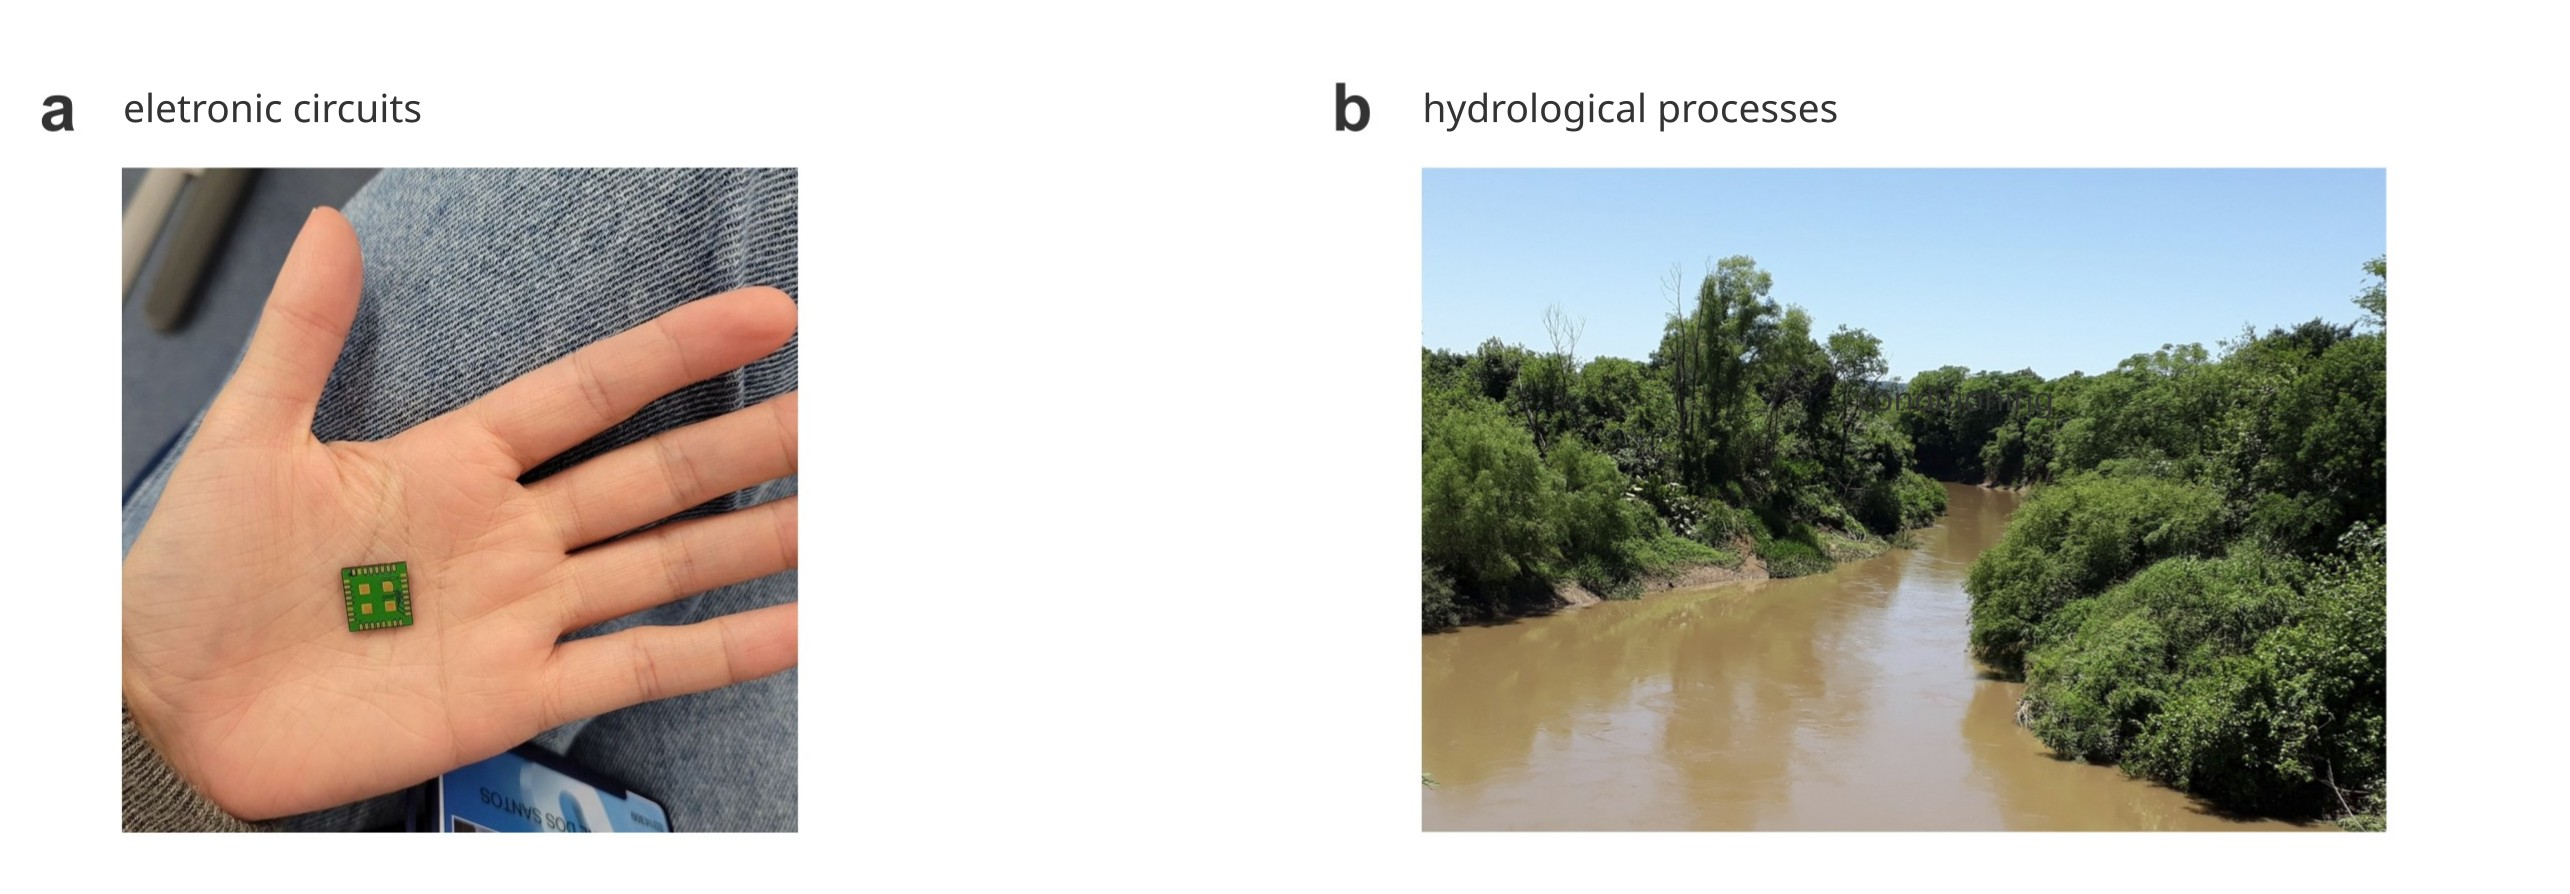
\includegraphics[width=0.95\linewidth]{fig_circuits_en.jpg}		
	\caption[From electronic circuits to hydrological processes]
	{\textbf{---\;From electronic circuits to hydrological processes.}
        \;\textbf{a.}\;---\;Applying a hydrological \gls{model} consists of \textit{literally} applying voltages to digital electronic circuits. The simulation results refer literally and objectively to the processing of the binary states of transistors. \;\textbf{b.}\;---\;Hydrological model users generally accept that the electronic results are a \textit{realistic representation}, albeit approximate, of various hydrological processes, whether it be rainfall infiltration, \gls{sf-runoff}, or river discharge. How is this possible? The photograph in (\textbf{a}) was kindly provided by electrical engineer Karina Kerne; the photograph in (\textbf{b}) was taken by the author on the bridge over the Pardinho River south of Lago Dourado, Santa Cruz do Sul, Rio Grande do Sul, Brazil.
	}
\label{fig:circuits}  % use qualitative label			
\end{figure}

\par Beven calls this common implicit philosophy among hydrological model users \textbf{\gls{prag-realism}}. He classifies this stance as naïve, demonstrating that the much-desired realistic representation, when taken seriously, becomes an extraordinary goal in light of the \textbf{\gls{uncert-empirical}} that exists in hydrological modeling. If water resource management genuinely wishes to build \textbf{\gls{ebp}}, scientific advice must adopt a \textit{critical stance} toward the use of models and their results. As highlighted by Ongaro and Andreoletti, uncertainty is a pervasive attribute in the decision-making process \cite{Ongaro2022}. In this context, they argue that the proper role of scientific authorities is to inform about empirical uncertainties so that other interest groups can deliberate on the ethical and political uncertainties at play. However, this critical stance is only possible from an explicit philosophical perspective, referred to here as \textbf{\gls{instrument}}, which brings to the fore several problems that need to be addressed before affirming the correspondence between electromagnetic fields in electronic circuits and hydrological processes in watersheds.

\par In this spirit, the aim of this chapter is to establish the instrumentalist philosophical foundations that will be explicitly used throughout this thesis. I will articulate the following issues from the Philosophy of Science: the \gls{problem-just}, Bayesian epistemology, the \gls{falseabilidade} of theories, the concept of paradigms, and the \gls{problem-subdet}. The ontology of models, which is also a relevant topic, will be addressed in the next chapter. For the purposes of this chapter, one must consider that \textbf{a \gls{model} is a symbolic vehicle of a theory}. The intention is not to exhaust the presented topics (as this would require writing many other theses!). On the contrary, this chapter should be understood as a panoramic view, as if we were standing atop a mountain. This \gls{analogy} is particularly useful, as the summit provides a good understanding of the landscape stretching below our feet. At the same time, it is a hostile territory. The air is thin, and we feel dizzy. Movement is complicated, possible only through labyrinths of trails surrounded by cliffs and caves. Care must be taken not to get lost and never return.

\section{The problem of justification} \label{sec:epis:justific}

\par \textbf{Epistemology} is the branch of Philosophy that investigates the nature of human knowledge itself. The epistemological question is: \textit{how is it possible to know something}? From this perspective, a \textbf{\gls{teoria}} is a \textit{universal statement} that provides a definitive explanation about a particular phenomenon. Thus, creating a \gls{teoria} is relatively easy. Someone might profess, for example, the \gls{teoria} that forest fairies are responsible for making household objects disappear, especially socks. We have a phenomenon (the disappearance of things) and a definitive explanation (the fairies). The difficult part, however, is \textit{justifying the truth} of a \gls{teoria}—the so-called \textbf{\gls{problem-just}}. Here, the epistemological question becomes a bit more complicated: \textit{how is it possible to know something \textbf{true}}? In the given example, if someone claims that, in fact, the dog is responsible for making the socks disappear, how can one defend the fairy \gls{teoria}? How do we separate the true from the false? The example of forest fairies might seem ridiculous at first glance. But just a few centuries ago, people were tortured and burned alive in public squares over issues like this (especially women accused of being witches). Even today, in fact, it is a very serious issue, with significant social and political implications. According to Daniel Kahneman, research in the field of psychology shows that humans exhibit numerous \textbf{cognitive biases} that compromise their ability to distinguish the true from the false \cite{kahneman2011}.

\par The epistemological problem of justifying theories was assimilated by two different philosophical schools of thought during the birth of the \textbf{scientific method} in modernity \cite{sep-rationalism-empiricism}. One of these schools, \textbf{\gls{rationalism}}, holds that \textit{Logic} must be the justification for the truth of theories. After all, it is clear that an incoherent explanation cannot be true. This position is commonly associated with Descartes (1596-1650), Spinoza (1632-1677), and Leibniz (1646-1716) — the so-called continental rationalists. René Descartes, one of the greatest rationalists of his time, propagated the notion that the senses are deceptive and elected reason as the guide for his opinions, establishing a program he called the \textit{method of doubt}. In his \textit{Discourse on the Method}\footnote{Descartes delves deeper into his ideas in \textit{Meditations}.}, he went so far as to doubt the existence of everything, claiming that reality could be indistinguishable from a mere dream \cite{descartes2008discurso}. With that, he concluded that the simple act of \textit{doubting} existence guarantees at least one absolute certainty: the existence of oneself\footnote{Descartes' idea that "I think, therefore I am" (\textit{cogito, ergo sum}) guarantees the existence of a \textit{Self} that asks questions. Descartes uses this to attempt to prove the existence of God as well. However, Descartes' proof of God is questionable, which can easily lead us to \textbf{solipsism}: the thesis that the \textit{Self} is alone, floating in the void, imagining a reality that fundamentally does not exist. After all, how can \textit{you}, the one reading this text, be certain that \textit{I}, the author, exist? How can you be sure that all your memories were not just created right now, at this very instant? And what if your entire life is nothing but an immaterial hallucination?}. The other philosophical school, \textbf{\gls{empiricism}}, argues that a \gls{teoria} is justified by \textit{empirical evidence}, that is, through a collection of direct observations of events and phenomena. This line of thought is associated with philosophers Locke (1632-1704), Hume (1711-1776), and Reid (1710-1796), the so-called British empiricists. Locke, for instance, became known for spreading the idea that all people are born equal, like a blank slate, a \textit{tabula rasa}, and acquire knowledge through experience, by interacting with their environment \cite{sep-locke}.


\par Although not exactly opposing, what these philosophical schools favor, in essence, are different methods of \textit{inference}. While rationalists prefer \textbf{\gls{infer-dedu}}, empiricists prefer \textbf{\gls{infer-indu}}. In the first case, statements are justified when they logically follow from their premises, that is, they are deduced \cite{laird2010}. For example, considering the premises that \say{\textit{all Gauchos like mate}} and that \say{\textit{Clara is a Gaucho}}, then we deduce that \say{\textit{Clara likes mate}}. Typically, the process of \gls{infer-dedu} follows a structure in which a conditional statement (if $S_1$ is true, then $S_2$ is also true) is followed by an \textit{antecedent} sentence, which can be either an affirmation (\textit{modus ponens}: $S_1$) or a negation (\textit{modus tollens}: $\neg S_1$), leading to the conclusion of the \textit{consequent} sentence. In the affirmative form (\textit{modus ponens}):
\begin{linenomath*}
    \begin{align*}
        S_1 \implies S_2 & \quad \textnormal{if someone is from the Pampas, then that person likes drinking mate} \\
        S_1 & \quad \textnormal{Clara is from the Pampas}\\
        \therefore\;S_2 & \quad \textnormal{therefore, Clara likes drinking mate}
    \end{align*}
\end{linenomath*}
\gls{infer-dedu} guarantees the truth of the consequent sentence as long as its antecedent premises are true. In the affirmative mode illustrated, it deduces \textit{singular statements} from \textit{universal statements}. \gls{infer-indu}, on the other hand, goes in the opposite direction. Empiricists seek to build theories (universal statements) by \textit{generalizing} from evidence (singular statements) obtained through empirical experience. This gives rise to the notion of a \textbf{\gls{hipotese}}: a draft of a \gls{teoria} to be \textit{confirmed} or \textit{verified} by evidence. For example, if we observe that the Gauchos we know like to drink mate, we can infer, by induction, that \textit{all} Gauchos must like mate. With a bit more caution and empirical rigor, we might eventually state that the \textit{probability} of any given Gaucho liking mate is high, since 99\% of respondents in a survey of a thousand Gauchos said that yes, they like to drink mate. For empiricists, the observation of phenomena justifies the construction of generalizations that are plausible or \textit{probable}.

\par Both lines of reasoning are problematic. The strict use of Logic as a justification for theories produces the \textbf{\gls{problem-regress}} \cite{cling2008}: if a statement $S_1$ is justified by another statement $S_2$ ($S_2 \implies S_1$), what justifies $S_2$? Perhaps statement $S_3$ justifies $S_2$, and statement $S_4$ justifies $S_3$, and so on, \textit{ad infinitum} ($\infty \implies ... \implies S3 \implies S_2 \implies S_1$). An alternative is to establish a circular chain of statements ($S_1 \implies S_2 \implies S_3 \implies S_1$), but this is, logically speaking, even worse than the previous situation, as ultimately the statements end up self-justifying. Infinite regress is easily noticed when children, being naturally curious, learn to ask \say{\textit{why?}}. One can stop the regress (or at least \textit{stop the questions}) by establishing fundamental truths, unquestionable axioms, as happens in Mathematics. But in Science, this only produces \textit{dogmatic} theories based on relatively arbitrary conventions, which are easy targets for empiricist criticism. On the other hand, using empirical experience as a justification for theories brings with it an insoluble problem, described by David Hume (1711-1776) and known today as the \textbf{\gls{problem-indu}}. \gls{infer-indu} is fragile because it is based on the \textbf{\gls{principio-uniform}}: the assumption that the regularities of nature observed in the past will be the same as those observed in the future. This assumption is the foundation of all Physics, after all, the laws observed today are often used to predict future events and reconstruct past events. Despite being intuitive, it is not possible to rationally justify the \gls{principio-uniform}. If we invoke the fact that it has always proven functional or correct, we fall into a circular, logically invalid argument that \textit{evokes the very \gls{principio-uniform} to justify the principle of uniformity} \cite{sep-induction-problem}. In other words, one cannot defend \gls{infer-indu} through an inductive argument! Thus, the \gls{principio-uniform} is ultimately the fundamental dogma of the empiricists\footnote{Hume's ideas inevitably lead us to \textbf{skepticism}. Beyond the \gls{problem-indu}, Hume argued that \textbf{causality} between phenomena is an imaginary concept, never \textit{directly} experienced in reality. Imagine a billiard ball colliding with another ball at rest. Then, the ball at rest begins to move as well. Newton would say that this happened \textit{because of} the law of conservation of motion. But this law requires several imagined theoretical concepts, such as mass and energy. What we can actually experience are events happening one after the other, but never the cause-and-effect connection between them. For Hume, \textit{this connection does not exist}.}.
    
\par The progress of modernity gradually reduced the intellectual rivalry between thinkers from the European continent and the British Isles. \gls{empiricism}, although revised and moderated, triumphed over \gls{rationalism} — especially after the work of Immanuel Kant (1724-1804). In his \textit{Critique of Pure Reason} (1781), this thinker proposes a synthesis between \gls{rationalism} and \gls{empiricism} \cite{silveira2002, weiss2017}. In it, Kant agrees with the empiricists — that empirical experience justifies knowledge — but makes a concession to \gls{rationalism}, establishing that theoretical concepts about the objects to be known are necessary \textit{a priori}. Without what he called \textbf{transcendental categories}, we cannot do much with the perceptions we collect about the external world. The hegemony of \gls{empiricism} in modernity culminated in the early 20th century with the philosophical movement of \textbf{\gls{positivismo}}. This movement established the common sense that scientific theories are \textit{verified} or \textit{confirmed} through the collection of observations and statistical analyses. However, this conception was surpassed in the mid-20th century, mainly due to the remarkable transformations in Physics. This reignited the debate about how Science justifies its theories and changes them in the long term, with new perspectives proposed by Karl Popper (1902-1994) and Thomas Kuhn (1922-1996), creating the conditions for the contemporary debate in the Philosophy of Science: \gls{realism-sci} and the purpose of Science.

\section{The process of confirmation} \label{sec:epis:bayes}

\par In the previous section, we saw that the empiricist school holds that a \gls{hipotese} represents a draft of a \gls{teoria} that must be \textit{confirmed} by empirical experience. In this sense, the ideas of the philosopher and statistician Thomas Bayes (1701-1761) provide a particularly useful method of \gls{infer-indu} for the confirmation of hypotheses through the mathematics of probabilities \cite{sep-epistemology-bayesian}, \cite{sprenger2019}. The central idea of the so-called \textbf{Bayesian epistemology} professes that knowledge is not an all-or-nothing matter, black or white, but presents subtleties, with various shades of gray between true and false. The reason for this stems from the recognition that empirical observations are inevitably subject to \textit{random noise}, meaning there is \textbf{\gls{uncert-stats}} in the sampled data. For this empiricist approach, the subtleties of knowledge consist in the \textbf{\gls{grau-convic}} in the truth of a \gls{hipotese}. This \gls{grau-convic} should be updated as favorable or unfavorable evidence is obtained through empirical experience.

\par Before proceeding, it will be useful to establish an intuitive example.

\par Consider that you are at the airport of a distant country, in the food court of a busy international terminal. You want to know if the person at the table in front of you will take the same flight as you to Brazil. With no information available, your \gls{grau-convic} in this \gls{hipotese} is relatively low, as there are dozens of flights scheduled from this terminal to various other countries. But if you suspect that the person is Brazilian, your \gls{grau-convic} increases — after all, your flight is likely full of other Brazilians. At the same time, caution is needed, as being Brazilian does not necessarily imply traveling to Brazil. Even if the person were not Brazilian, there would still be a small chance that they are traveling to Brazil on the same flight as you, for tourism or business. One thing is certain: \textit{favorable evidence that the person is Brazilian will lead you to update your degree of conviction}. Bayesian epistemology articulates how to do this in a mathematically precise way.

\par A good starting point to formalize the concept of \gls{grau-convic} in terms of probabilities is to note that a given \gls{hipotese} $H$ and its favorable evidence $E$ are distributed in a \textbf{\gls{espaco-possib}} $\Omega$. From a Bayesian perspective, each of these possibilities is assigned a \gls{grau-convic}, which can be considered probabilistic as long as they are \textit{mutually exclusive} (they cannot both be true at the same time) and \textit{jointly exhaustive} (at least one of them is true). Given these conditions, the \textbf{\gls{princip-prob}} is observed based on the following axioms:
\begin{itemize}
    \item \textbf{Non-negativity}. The probability of a given possibility $A$ must be a non-negative real number: $P(A) \geq 0$;
    \item \textbf{Normalization}. The probabilities of all possibilities must sum to one: $P(\Omega) = 1$, and;
    \item \textbf{Additivity}. Because they are incompatible, the probability of two possibilities $A$ and $B$ is the sum of their individual probabilities: $P(A \cup B ) = P(A) + P(B)$.
\end{itemize}

\par In the airport example, there are four possibilities: the person is Brazilian and on the same flight ($E$ is true and $H$ is true); the person is Brazilian and not on the same flight ($E$ is true and $H$ is false); the person is not Brazilian and on the same flight ($E$ is false and $H$ is true); and the person is not Brazilian and not on the same flight ($E$ is false and $H$ is false). This \gls{espaco-possib} can be more easily visualized through a table with illustrative numbers, as in Table\,\ref{tbl:bayes-aeroporto}. So, consider that in the international terminal, there are 200 scheduled flights (only one of them to Brazil) and that each plane carries 500 passengers. In total, there are 100,000 passengers circulating in the terminal. Additionally, there are 800 Brazilians in the terminal, with 450 on your flight and another 350 with other destinations.
\begin{table}[ht]
     % placed on top of page    
    \centering	
    \small
    \sffamily
    \begin{tabular}{ l  c  c  c} % preset number of columns and alignment
       & \textbf{same flight ($H$)} & \textbf{different flight ($\neg H$)} & totals\\  
        \hline
        \textbf{is Brazilian ($E$)} & 450 & 350 & 800\\
        \textbf{is not Brazilian ($\neg E$)} & 50 & 99150 & 99200\\
        \hline
        totals & 500 & 99500 & 100000\\
    \end{tabular}
    \caption[Possibility space for the airport example]{Possibility space for the airport example. The numbers represent the distribution of passengers in the different combinations between \gls{hipotese} $H$ (on the same flight) and evidence $E$ (nationality is Brazilian)}
    \label{tbl:bayes-aeroporto}
\end{table} 

By inspecting the table, we can easily see that the probability of your \gls{hipotese} being true, that any given passenger is on your flight, is $P(H) = 0.005$ (0.5%), as $500 / 100000 = 0.005$. In Bayesian jargon, this is the \textbf{\gls{prior}}. However, the evidence that this person might be Brazilian changes everything. Now, the probability of your \gls{hipotese} being true given that the evidence is true is $P(H | E) = 0.56$ (56%), as $450 / 800 = 0.56$. In Bayesian jargon, this is the \textbf{\gls{posterior}}. The \textbf{\gls{bayes-theorem}} formalizes this reasoning:
\begin{linenomath*}
\begin{equation}
\label{eq:bayes}
    P(H | E) = \frac{P(H) \cdot P(E | H)}{P(E)}
\end{equation}
\end{linenomath*}
Where $P(H | E)$ is the probability of \gls{hipotese} $H$ being true given that evidence $E$ is true (posterior probability); $P(H)$ is the probability of \gls{hipotese} $H$ being true (prior probability); $P(E | H)$ is the probability of evidence $E$ being true given that \gls{hipotese} $H$ is true, called the \textbf{\gls{likelihood}}, and $P(E)$ is the probability of the evidence being true under all possibilities. In the case of the airport:
\begin{linenomath*}
\begin{equation*}
    P(H | E) = \frac{\frac{500}{100000} \cdot \frac{450}{500}}{\frac{800}{100000}} = \frac{450}{800} = 0.56\,(56\%)
\end{equation*}
\end{linenomath*}
What Bayes' Theorem tells us is that the estimate of the probability of the \gls{hipotese} being true given favorable evidence must take into account both the \gls{espaco-possib} reduced \textit{by the favorable evidence} (in this case, the fact that there are few Brazilians in the international terminal) and the chance \textit{that the evidence does not guarantee the hypothesis} (in this case, the fact that not everyone on your flight is Brazilian). Or simply:
\begin{linenomath*}
\begin{equation*}
    \text{Posterior} = \text{Prior} \times \text{Likelihood} \div \text{Evidence}
\end{equation*}
\end{linenomath*}

\par The update of the \gls{grau-convic} is only possible \textit{provided that} the evidence favorable to the \gls{hipotese} is true. For this reason, this is called the \textbf{\gls{princip-cond}} of Bayesian epistemology. In the airport example, everything is quite clear because the absolute numbers of passengers were provided in the table. The probabilities calculated this way are objective, based on the \textit{frequency} of each set in the \gls{espaco-possib} $\Omega$. But in a practical situation, we usually only have access to the degrees of conviction in the \gls{espaco-possib} $\Omega$, which must change as new evidence is obtained. To remain consistent with the axioms of probabilism, conditioning or \textbf{\gls{conditioning}} \footnote{The terms \textit{conditioning} and \textit{conditionalization} will be used equivalently here.} with the evidence must \textit{zero out}, \textit{rescale}, and \textit{normalize} the probability values. In the airport example, when we find out that the person in the airport is definitely Brazilian, we must zero out the probabilities that they are not Brazilian, which implies proportionally rescaling the probability of the other possibilities and \textit{normalizing their values} so that their sum equals one, as $P(\Omega) = 1$. On the other hand, if we only infer that the person at the table ahead speaks Portuguese (perhaps by reading a book), this is not enough to zero out the probability that they are not Brazilian (after all, other nationalities also speak Portuguese!).

\begin{table}[t]
     % placed  here
    \centering	
    \small
    \sffamily
    \rowcolors{2}{white}{rowgray}
    \begin{tabular}{ l c c c c c } % preset number of columns and alignment
        \toprule
        \textbf{Hypothesis \textit{i}} & \textbf{$P(H_i)$} & \textbf{$P(E | H_i)$} & \textbf{$P(H_i) \cdot P(E | H_i)$} & \textbf{$P(H_i | E)$}\\ 
        \midrule
        $H_1$: $X < x_1$ & 0.143 & 0.008 & 0.001 & 0.008\\ 
        $H_2$: $x_1 \leq X < x_2$ & 0.143 & 0.026 & 0.004 & 0.026\\ 
        $H_3$: $x_2 \leq X < x_3$ & 0.143 & 0.084 & 0.012 & 0.084\\ 
        $H_4$: $x_3 \leq X < x_4$ & 0.143 & 0.171 & 0.024 & 0.171\\ 
        $H_5$: $x_4 \leq X < x_5$ & 0.143 & 0.208 & 0.03 & 0.208\\ 
        $H_6$: $x_5 \leq X < x_6$ & 0.143 & 0.275 & 0.039 & 0.275\\ 
        $H_7$: $X \geq x_6$ & 0.143 & 0.227 & 0.032 & 0.227\\ 
        \midrule
        totals & 1.0 & 1.0 & 0.14 & 1.0\\
        \bottomrule
    \end{tabular}
    \caption[Objective \gls{conditioning} example]{
    Illustrative example of the \gls{conditioning} of the probability distribution of a random variable $X$. In this case, the prior distribution $P(H)$ was defined as uniform by observing the \gls{princip-indif} (objective Bayesianism).
    }
    \label{tbl:objective}
\end{table} 

\begin{table}[t]
     % placed  here
    \centering	
    \small
    \sffamily
    \rowcolors{2}{white}{rowgray}
    \begin{tabular}{ l  c  c  c  c c} % preset number of columns and alignment
        \toprule
        \textbf{Hypothesis \textit{i}} & \textbf{$P(H_i)$} & \textbf{$P(E | H_i)$} & \textbf{$P(H_i) \cdot P(E | H_i)$} & \textbf{$P(H_i | E)$}\\ 
        \midrule
        $H_1$: $X < x_1$ & 0.227 & 0.008 & 0.002 & 0.022\\ 
        $H_2$: $x_1 \leq X < x_2$ & 0.273 & 0.026 & 0.007 & 0.088\\ 
        $H_3$: $x_2 \leq X < x_3$ & 0.229 & 0.084 & 0.019 & 0.236\\ 
        $H_4$: $x_3 \leq X < x_4$ & 0.146 & 0.171 & 0.025 & 0.306\\ 
        $H_5$: $x_4 \leq X < x_5$ & 0.082 & 0.208 & 0.017 & 0.208\\ 
        $H_6$: $x_5 \leq X < x_6$ & 0.036 & 0.275 & 0.01 & 0.12\\ 
        $H_7$: $X \geq x_6$ & 0.008 & 0.227 & 0.002 & 0.022\\ 
        \midrule
        totals & 1.0 & 1.0 & 0.08 & 1.0\\
        \bottomrule
    \end{tabular}
    \caption[Subjective \gls{conditioning} example]{
    Another illustrative example of \gls{conditioning} of the probability distribution of a random variable $X$. In this case, the prior distribution $P(H)$ was defined subjectively, by expert opinion (subjective Bayesianism).
    }
    \label{tbl:subjective}
\end{table}

\par The \gls{princip-cond} allows for the application of Bayes' Theorem to a finite number of $N$ hypotheses $H_1$, ..., $H_N$, as long as they are mutually exclusive and collectively exhaustive possibilities. In this case, Bayes' Theorem takes the following form:
\begin{linenomath*}
\begin{equation}
\label{eq:bayes-finite}
    P(H_i | E) = \frac{P(H_i) \cdot P(E | H_i)}{\sum_{j=1}^{N}P(E | H_j) \cdot P(H_j)}
\end{equation}
\end{linenomath*}
The denominator in this equation is a constant that plays the role of normalizing the probability values, ensuring that $P(\Omega) = 1$. Here, it is noted that normalization provides an opportunity to assign \textit{non-probabilistic} degrees of conviction to the \gls{likelihood} $P(E | H)$ without violating the \gls{princip-prob}, as long as they are non-negative values. In other words, the \gls{likelihood} $P(E | H)$ can be interpreted as a \textit{weight} given by the evidence. If this is the case, the notation for \gls{likelihood} should be modified to an \textbf{informal \gls{likelihood} function}, denoted by $\mathcal{L}(E|H)$\footnote{This is the basis of the \acrfull{glue} method for uncertainty analyses, introduced in the next chapter}. Either way, the posterior distribution of a random variable must be conditioned by an empirically estimated probability (or weight) distribution. To do this, it is necessary to discretize the values of the variable into $N$ intervals, which are the hypotheses $H_1$, ..., $H_N$ in Equation \eqref{eq:bayes-finite}. For each \gls{hipotese} $H_i$, its \gls{prior} $P(H_i)$ must first be assigned. Next, empirical evidence must be obtained to derive the \gls{likelihood} $P(E | H_i)$ for each \gls{hipotese}. The \gls{posterior} of each \gls{hipotese} is then conditioned through the application of Equation \eqref{eq:bayes-finite}. Finally, if we consider the posterior distribution obtained as the prior distribution for the next stage, the confirmation of the probability distribution of the variable occurs incrementally as new evidence accumulates. Table \ref{tbl:objective} shows an example of the \gls{conditioning} of the probability distribution of a random variable $X$, which in this case was divided into seven discrete intervals defined by thresholds $x_1, ..., x_6$.

\par A controversial issue in the \gls{conditioning} process is the definition of prior probabilities in the very first stage when there is still no evidence. In the case of Table \ref{tbl:objective}, what justifies the \gls{prior} distribution $P(H_i)$ being uniform? This is the so-called \textbf{\gls{problem-priors}} in Bayesian epistemology, which divides the field into two main branches of Bayesianism: the \textit{subjective} and the \textit{objective}. To proceed, one must decide between the two. On the one hand, the \textbf{\gls{bayes-sub}} branch accepts any \gls{prior} distribution as long as it does not violate the \gls{princip-prob}. The obvious problem here is that the posterior distribution may become more sensitive to the values of the prior distribution than to the evidence itself, as demonstrated in Table \ref{tbl:subjective}. Figure \ref{fig:bayes} clearly shows the difference between the posterior results $P(H | E)$ between Tables \ref{tbl:objective} and \ref{tbl:subjective}, even though exactly the same \gls{likelihood} distribution $P(E | H)$ was used for the \gls{conditioning}. Defenders of this branch argue that it is legitimate for different subjective opinions to be compared objectively. Moreover, if the evidence is consistent, divergent opinions about the prior distribution become irrelevant in the long run, dissipating during successive \gls{conditioning} stages. On the other hand, the \textbf{\gls{bayes-obj}} branch prefers to eliminate any bias when defining the prior distribution. To this end, the \textbf{\gls{princip-indif}} is recommended: the \gls{grau-convic} in two or more hypotheses should be equal in the absence of sufficient reasons to the contrary. In the case of Table \ref{tbl:objective}, there may not be enough reasons to differentiate the values of $P(H_i)$, which is why a uniform distribution was adopted. This principle may seem natural, but it is nothing more than an arbitrary convention: in the face of complete ignorance, any \gls{prior} distribution is equally probable, with the uniform distribution being, in fact, an extremely specific case.

% figure
\begin{figure}[t!] % place figure in the page
	\centering				
	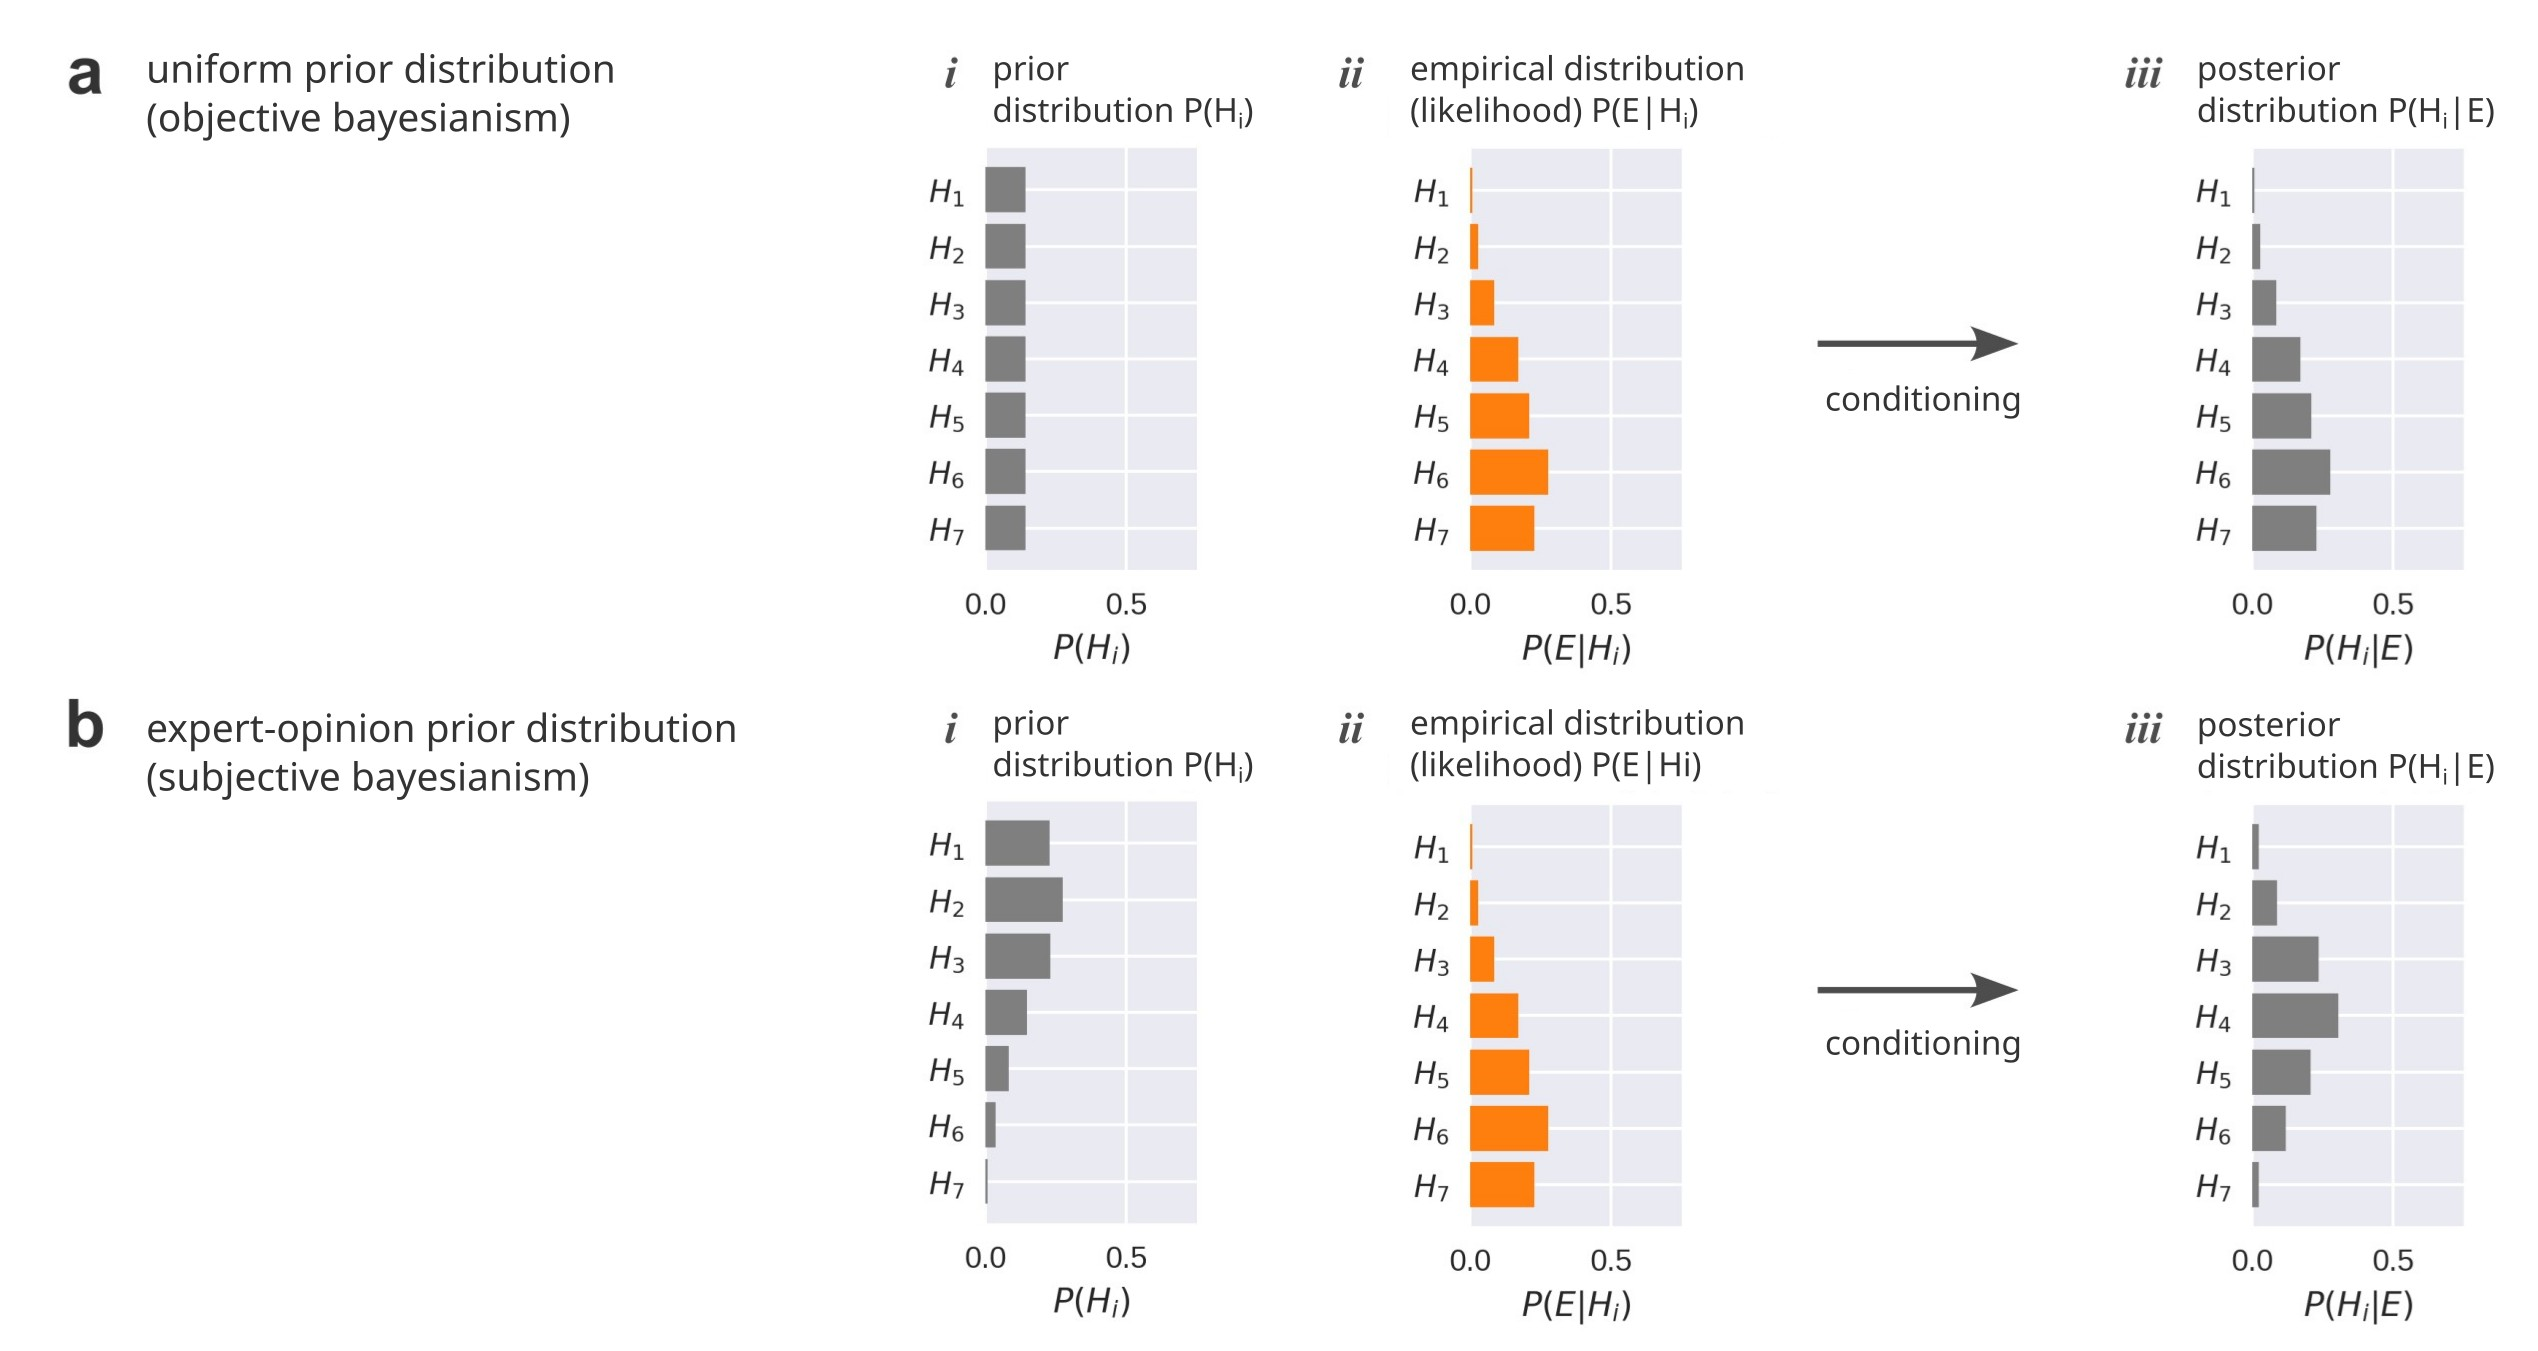
\includegraphics[width=0.95\linewidth]{fig_bayes_en.jpg}		
	\caption[Example of Bayesian conditioning]
	{\textbf{---\;Conditioning the prior distribution of a random variable.}
        This visually presents the illustrative data from Tables \ref{tbl:objective} and \ref{tbl:subjective}. In both cases, the evidence is the same; what changes are the assumptions used in the prior distribution. \;\textbf{a}\;---\;Uniform distribution, considering the \textit{principle of indifference} of \gls{bayes-obj}. \;\textbf{b}\;---\;Distribution defined by opinion, a practice considered valid in \gls{bayes-sub}.  
	}
\label{fig:bayes}  % use qualitative label			
\end{figure}


\par Another open issue in the \gls{conditioning} process is how to obtain the \gls{likelihood} $P(E | H)$ from the evidence. After all, without precise details about the entire \gls{espaco-possib} $\Omega$, as in the airport example, the evidence usually consists of sampled data that does not automatically translate into probabilities. This issue becomes even more pronounced in the case of a continuous random variable when we seek to estimate a probability distribution from the available data. Similar to the \gls{problem-priors}, the solution to this question requires a decision-making process, which involves establishing a set of assumptions about \textit{the behavior of random noise}\footnote{An ironic fact about the Bayesian approach is that the \gls{hipotese} about the behavior of the noise can only be justified through logic, never by the evidence, under penalty of entering an infinite regression of decisions about the noise of the noise. After all, to justify the \gls{hipotese} about random noise based on evidence, we would need to repeat the Bayesian method \textit{ad infinitum}, evaluating the noise of the noise, and the noise of the noise of the noise, and so on.}. In this direction, a particularly useful example for our future discussion on hydrological models is the fitting of mathematical curves that relate two phenomena, such as in the case of the \textbf{\gls{rating-curve}} that describes discharge as a function of the observed level at a river section (see Highlight \ref{box:rating-curve}). In this case, the mathematical curve represents the \gls{hipotese}, or \textbf{\gls{model}}, for which we are interested in knowing the \gls{grau-convic}. A general relationship for this problem is as follows \cite{Box1979}:
\begin{linenomath*}
\begin{equation}
\label{eq:bayes-model}
    O(x, t) = M(x, t, \Theta) + \varepsilon(x, t)
\end{equation}
\end{linenomath*}
In which $O(x, t)$ is the empirical observation obtained at the independent variable $x$ and time $t$; $M(x, t, \Theta)$ are the predictions of the \gls{model} $M$ at $x,t$ given the parameter vector $\Theta$, and; $\varepsilon(x, t)$ is the \textbf{error}\footnote{Also referred to as \textbf{residual}.} of the empirical observation at $x,t$. Of course, in this context, the random variables of interest for estimating the \gls{likelihood} of the \gls{model} $M$ are the \gls{parameters} $\Theta$ themselves. A typical set of assumptions\footnote{The introduction of bias, temporal autocorrelation, and other distributions can also be made within a mathematically formal, albeit more intricate, framework.} about the behavior of random noise is that the error $\varepsilon$ exhibits:
\begin{enumerate}
    \item zero mean, i.e., $\mu_{\varepsilon} = 0$;
    \item constant (stable) variance $\sigma_{\varepsilon}^2$;
    \item independence over time, and;
    \item normal distribution: $p(\varepsilon) = \frac{1}{\sigma_{\varepsilon} \sqrt{2\pi}}e^{-(\varepsilon-\mu_{\varepsilon})^2/{(2\sigma_{\varepsilon}^2)}}$, where $\mu_{\varepsilon}$ is the error mean (zero) and $\sigma_{\varepsilon}$ is the standard deviation of the error.
\end{enumerate}
\par The rational justification for considering the normal distribution is based on the \textbf{\gls{theorem-central-limit}}, which states that the sample mean of any population is normally distributed\footnote{What this theorem means is that sums of random numbers (note that the mean is a sum) tend to naturally produce the normal curve pattern simply by combining high values with low values. For example, consider rolling a fair six-sided die. The probability of each top face showing one of the values from the set $\{1, 2, 3, 4, 5, 6\}$ is the same, $1/6$. However, the probability of the \textit{mean} of the values sampled in $n$ rolls tends to be much higher among intermediate values as $n$ increases, since high values are offset by low values. This is the fact that produces the bell-shaped pattern modeled by the normal curve.}. Thus, the problem of the \gls{likelihood} of the \gls{parameters} $\Theta$ is resolved by estimating the population variance of the error $\sigma^2_\varepsilon$ by its sample variance, which is defined as $s^2_{\varepsilon} = \frac{1}{df}\sum_{i=1}^{n}({\varepsilon_i - \bar{\varepsilon}})^2$, where $\bar{\varepsilon}$ is the sample mean of the error; $n$ is the sample size, and; $df$ is the degrees of freedom\footnote{$df = n-2$ for models with two \gls{parameters}.} \cite{graybill1994}. The error $\varepsilon_i$ of each $n$ observation is the difference between the observation $O_i$ and the prediction of the model curve $M_i$ defined by the \gls{parameters} $\Theta$ adjusted with optimization techniques, such as the least squares method. Next, the uncertainty associated with the variance of the error must be assimilated in some way by the \gls{parameters} $\Theta$. For linear models, this can be done analytically, based on the principles of linear combination of random variables. A robust alternative, applicable to models in general, is the \textbf{\gls{monte-carlo}} method. In this method, numerous \textit{resamplings} of the error $\varepsilon$ are performed, i.e., simulations of statistically equivalent realizations\footnote{In the case of small samples, with $n < 30$, the error $\varepsilon$ should be simulated using the Student’s $t$ distribution with $n-1$ degrees of freedom.}. For each simulation, new values for the \gls{parameters} $\Theta$ are adjusted using optimization techniques. Thus, the database generated by these simulations allows the estimation of the empirical probability distribution of the \gls{parameters} $\Theta$ of the \gls{model} $M(x, t, \Theta)$, which can finally be used in the \gls{conditioning} process.

% figure
\begin{figure}[t!] % place figure in the page
	\centering				
	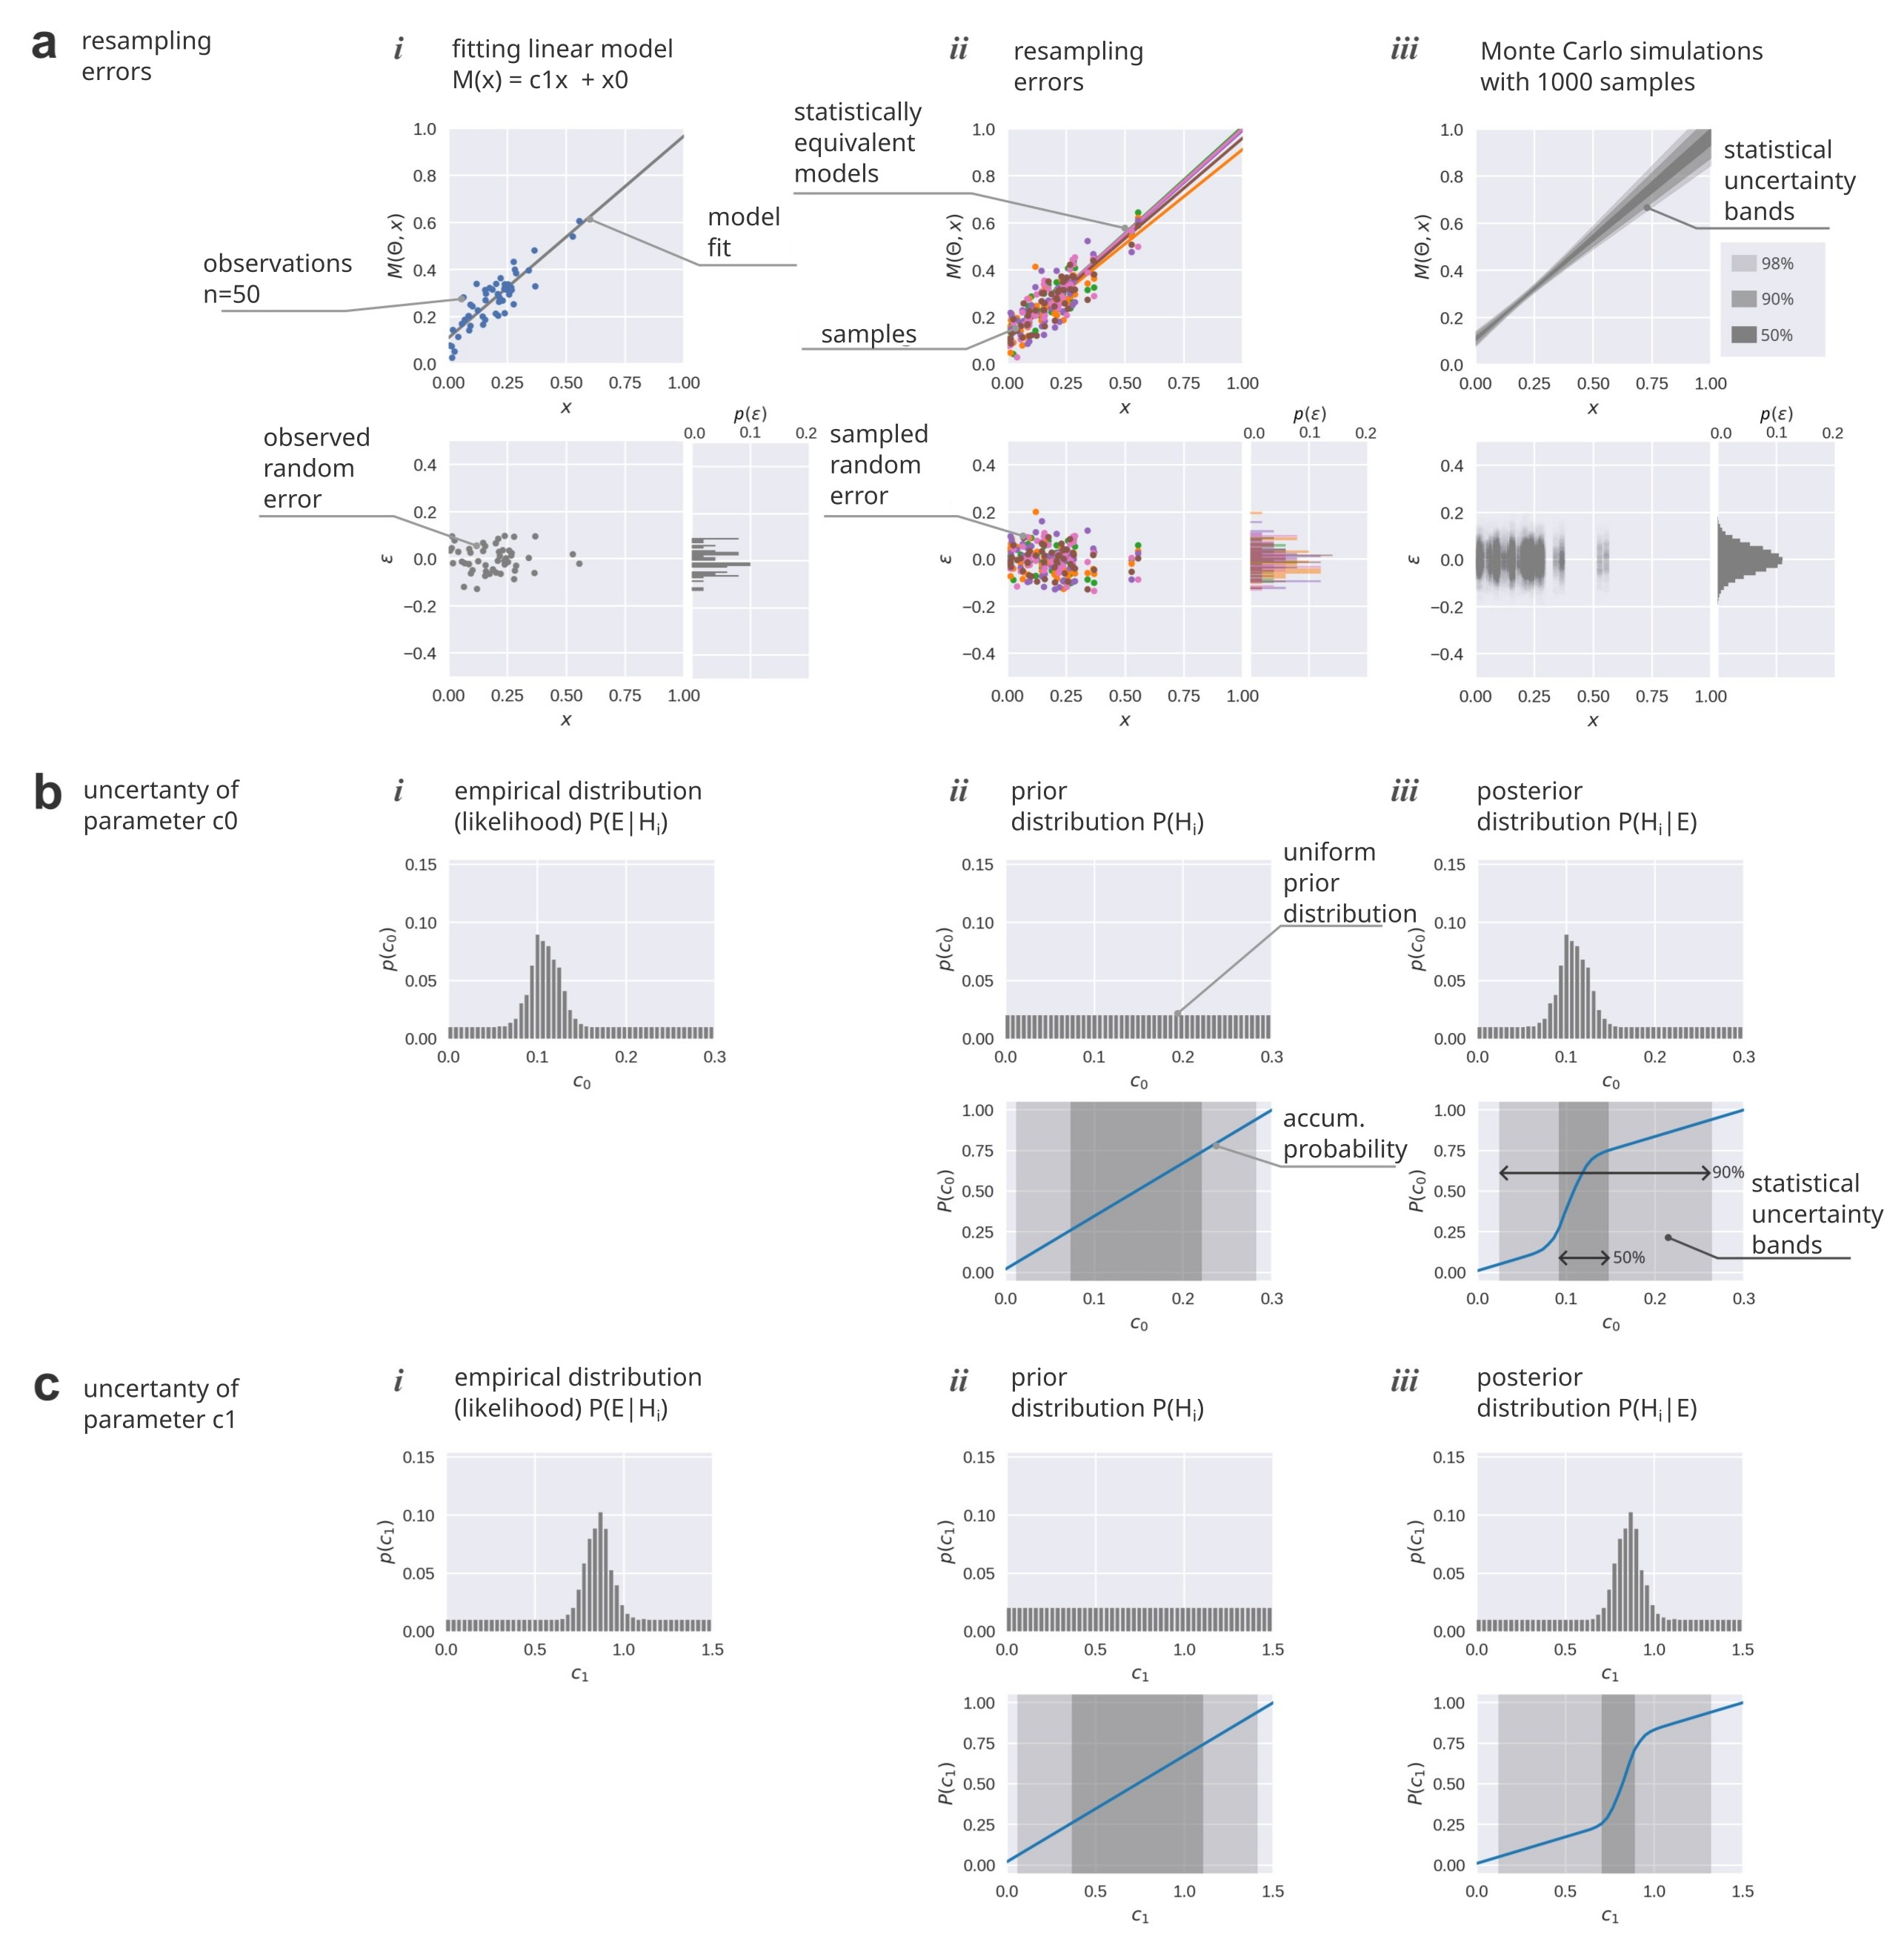
\includegraphics[width=0.95\linewidth]{fig_montecarlo_s1_en.jpg}		
	\caption[First stage of \gls{conditioning} of a linear \gls{model}]
	{\textbf{---\;First stage of \gls{conditioning} of a linear \gls{model} of the type $M(x, \Theta) = c_{1}x + c_{0}$.}
        \;\textbf{a}\;---\;Fitting a linear \gls{model} using the least squares method. This first fit allows estimating the behavior of the error $\varepsilon$ (detail a.\textit{\textrm{i}}.). If the assumptions about the error are met, numerous error resamplings are performed (\gls{monte-carlo}, details a.\textit{\textrm{ii}}. and a.\textit{\textrm{iii}}). For each resampling, new models are fitted. The resampling database allows the estimation of the empirical probability distribution of the parameters $c_0$ and $c_1$.\;\textbf{b}\;---\;Application of Bayes' Theorem to obtain the posterior distribution of parameter $c_0$ (detail b.\textit{\textrm{iii}}.). The empirical distribution (detail b.\textit{\textrm{i}}.) was obtained from the results of the Monte Carlo simulation.\;\textbf{c}\;---\;Application of Bayes' Theorem to obtain the posterior distribution of parameter $c_1$ (detail c.\textit{\textrm{iii}}.). The empirical distribution (detail c.\textit{\textrm{i}}.) was obtained from the results of the Monte Carlo simulation. In both cases, the prior distribution was considered uniform (b.\textit{\textrm{ii}}.; c.\textit{\textrm{ii}}.).
	}
\label{fig:bayes_s1}  % use qualitative label			
\end{figure}

% figure
\begin{figure}[t!] % place figure in the page
	\centering				
	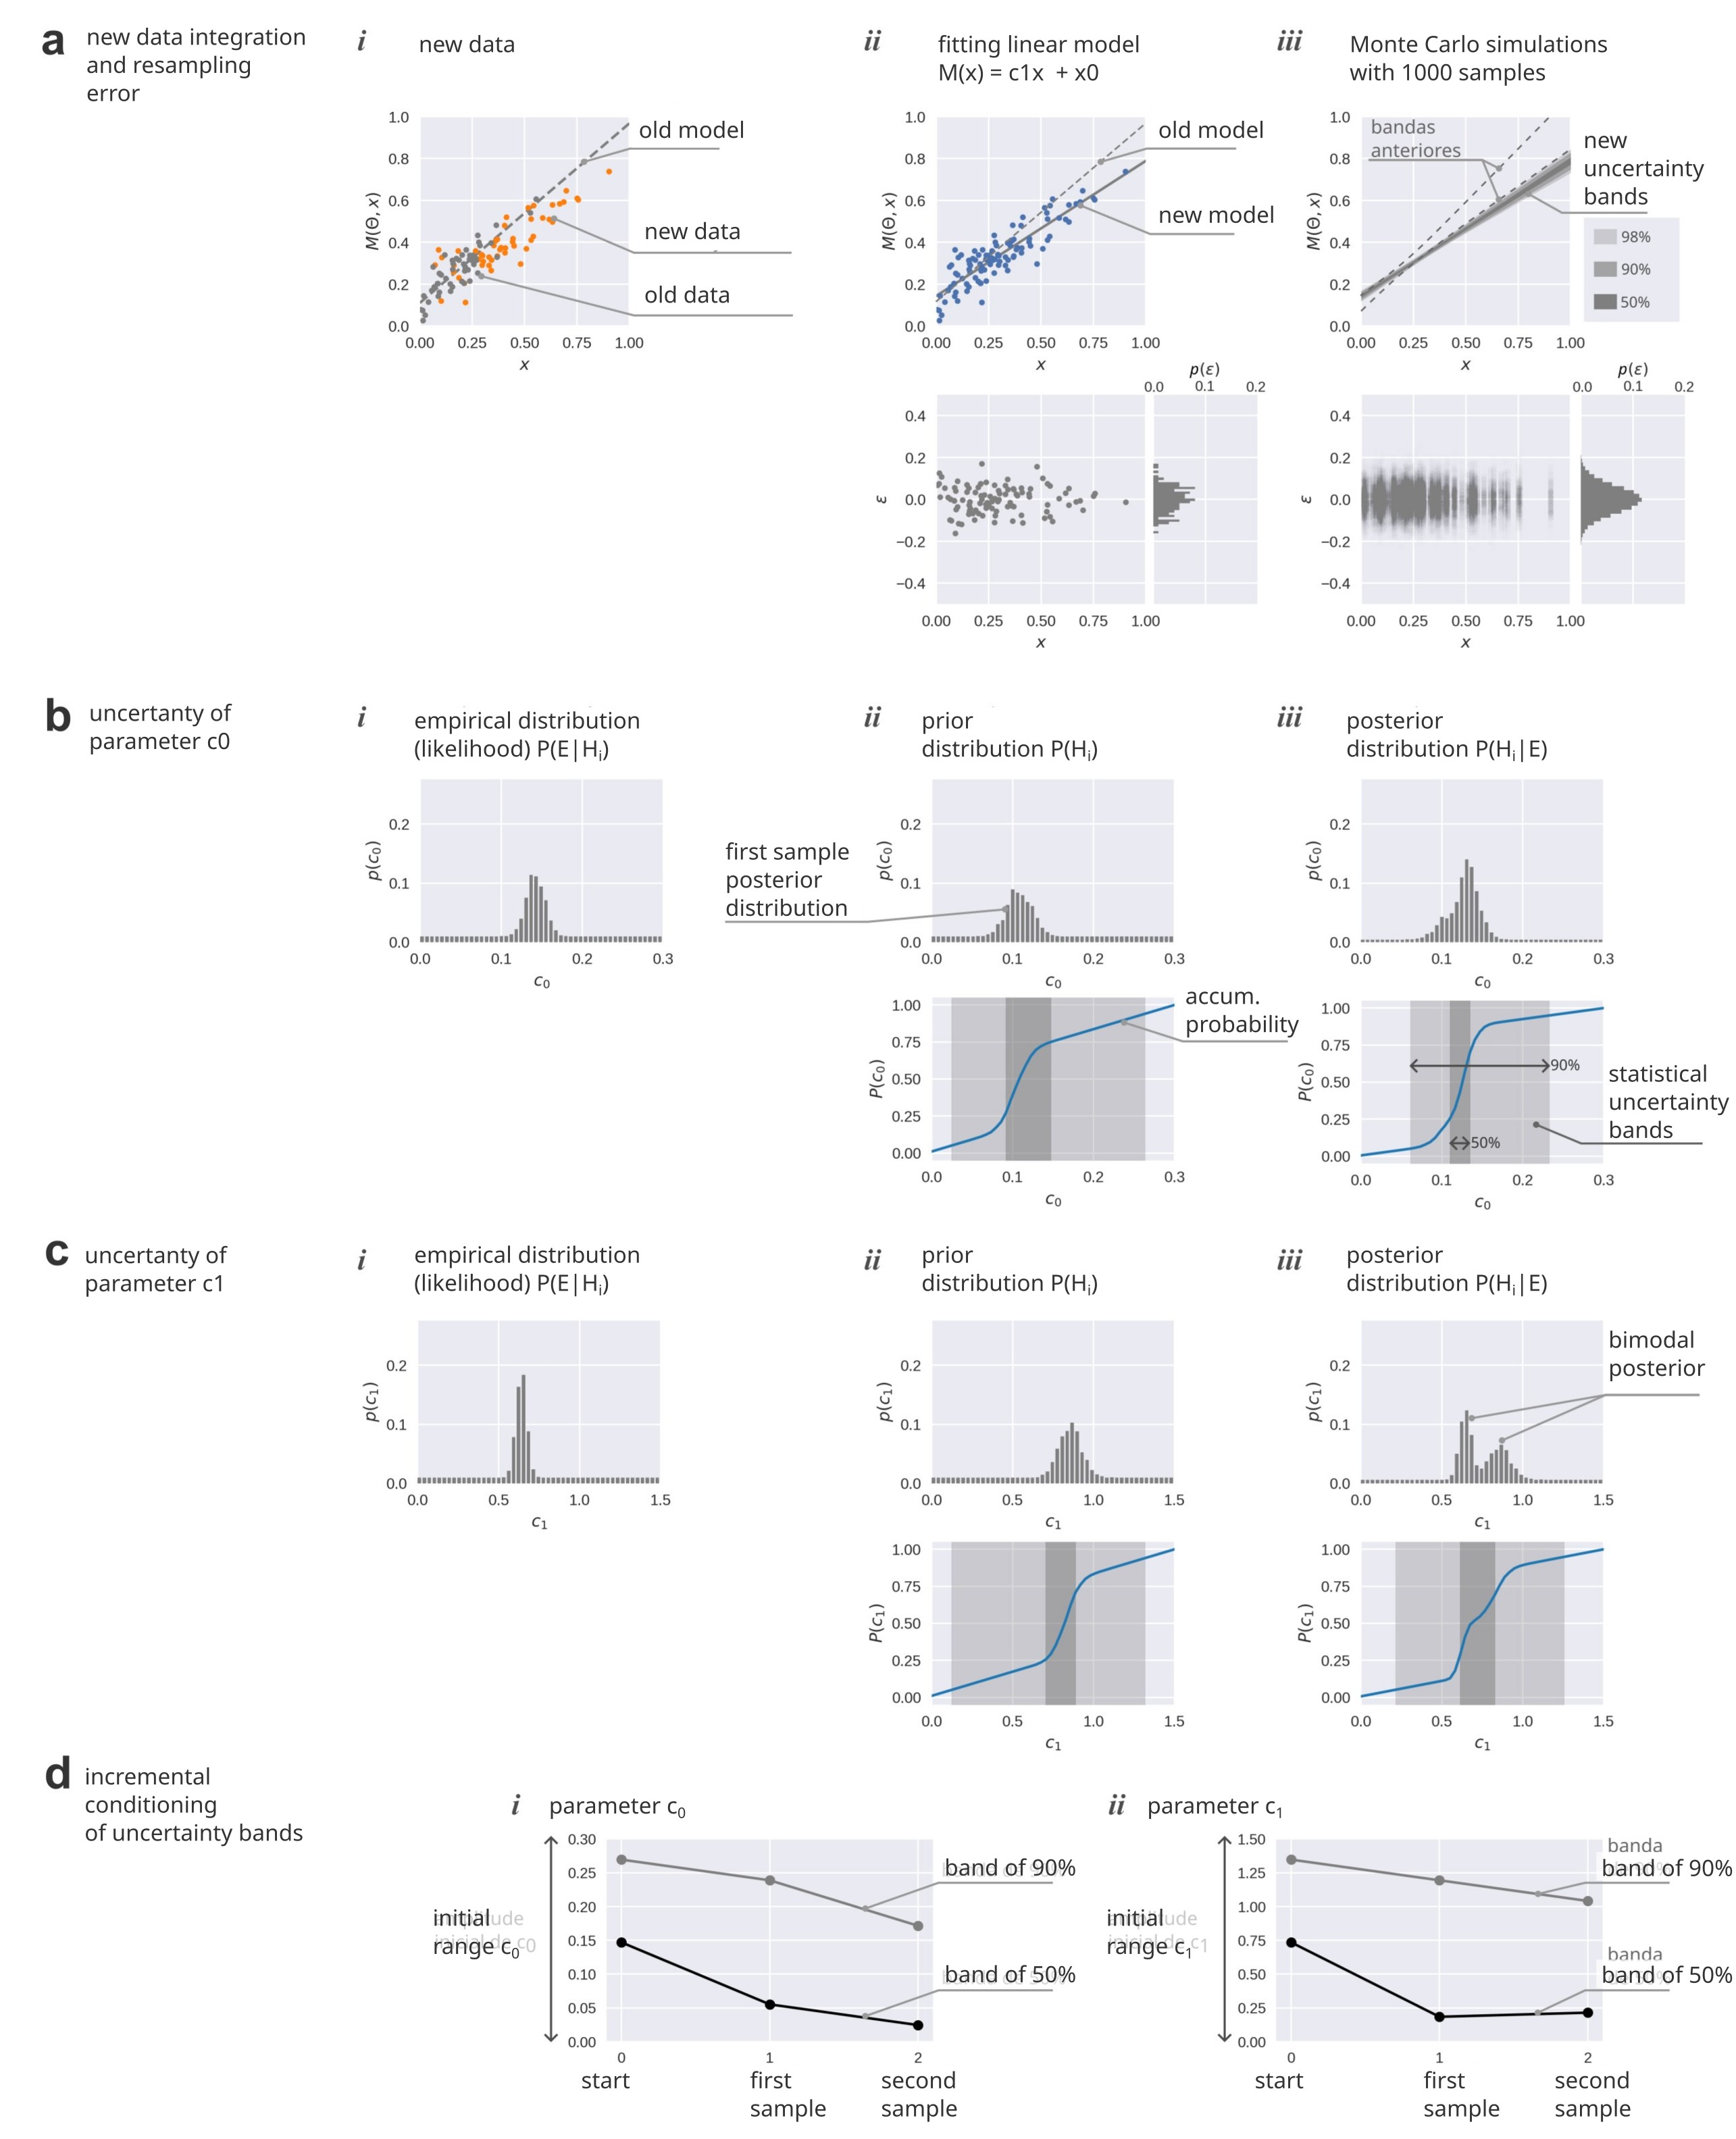
\includegraphics[width=0.95\linewidth]{fig_montecarlo_s2_en.jpg}		
	\caption[Second stage of \gls{conditioning} of a linear \gls{model}]
	{\textbf{---\;Second stage of \gls{conditioning} of a linear \gls{model} of the type $M(x, \Theta) = c_{1}x + c_{0}$.}
        \;\textbf{a}\;---\;Second stage of \gls{conditioning}. The same procedures are carried out as in the first stage, with the difference that new data obtained is integrated with previous observations and that the prior distribution used is the posterior distribution from the first stage.\;\textbf{b}\;---\;Application of Bayes' Theorem to obtain the posterior distribution of parameter $c_0$.\;\textbf{c}\;---\;Application of Bayes' Theorem to obtain the posterior distribution of parameter $c_1$.\;\textbf{d}\;---\;Analysis of the uncertainty bands of the parameters as new samples are taken. The uncertainty bands of the model's predictions and parameters have been reduced, except for the 50\% uncertainty band in the second stage of parameter $c_1$. This occurred because the evidence in the second sampling is highly inconsistent with those obtained in the first sampling, resulting in a bimodal posterior distribution (detail c.\textit{\textrm{iii}}.).
	}
\label{fig:bayes_s2}  % use qualitative label			
\end{figure}

% figure
\begin{figure}[t!] % place figure in the page
	\centering				
	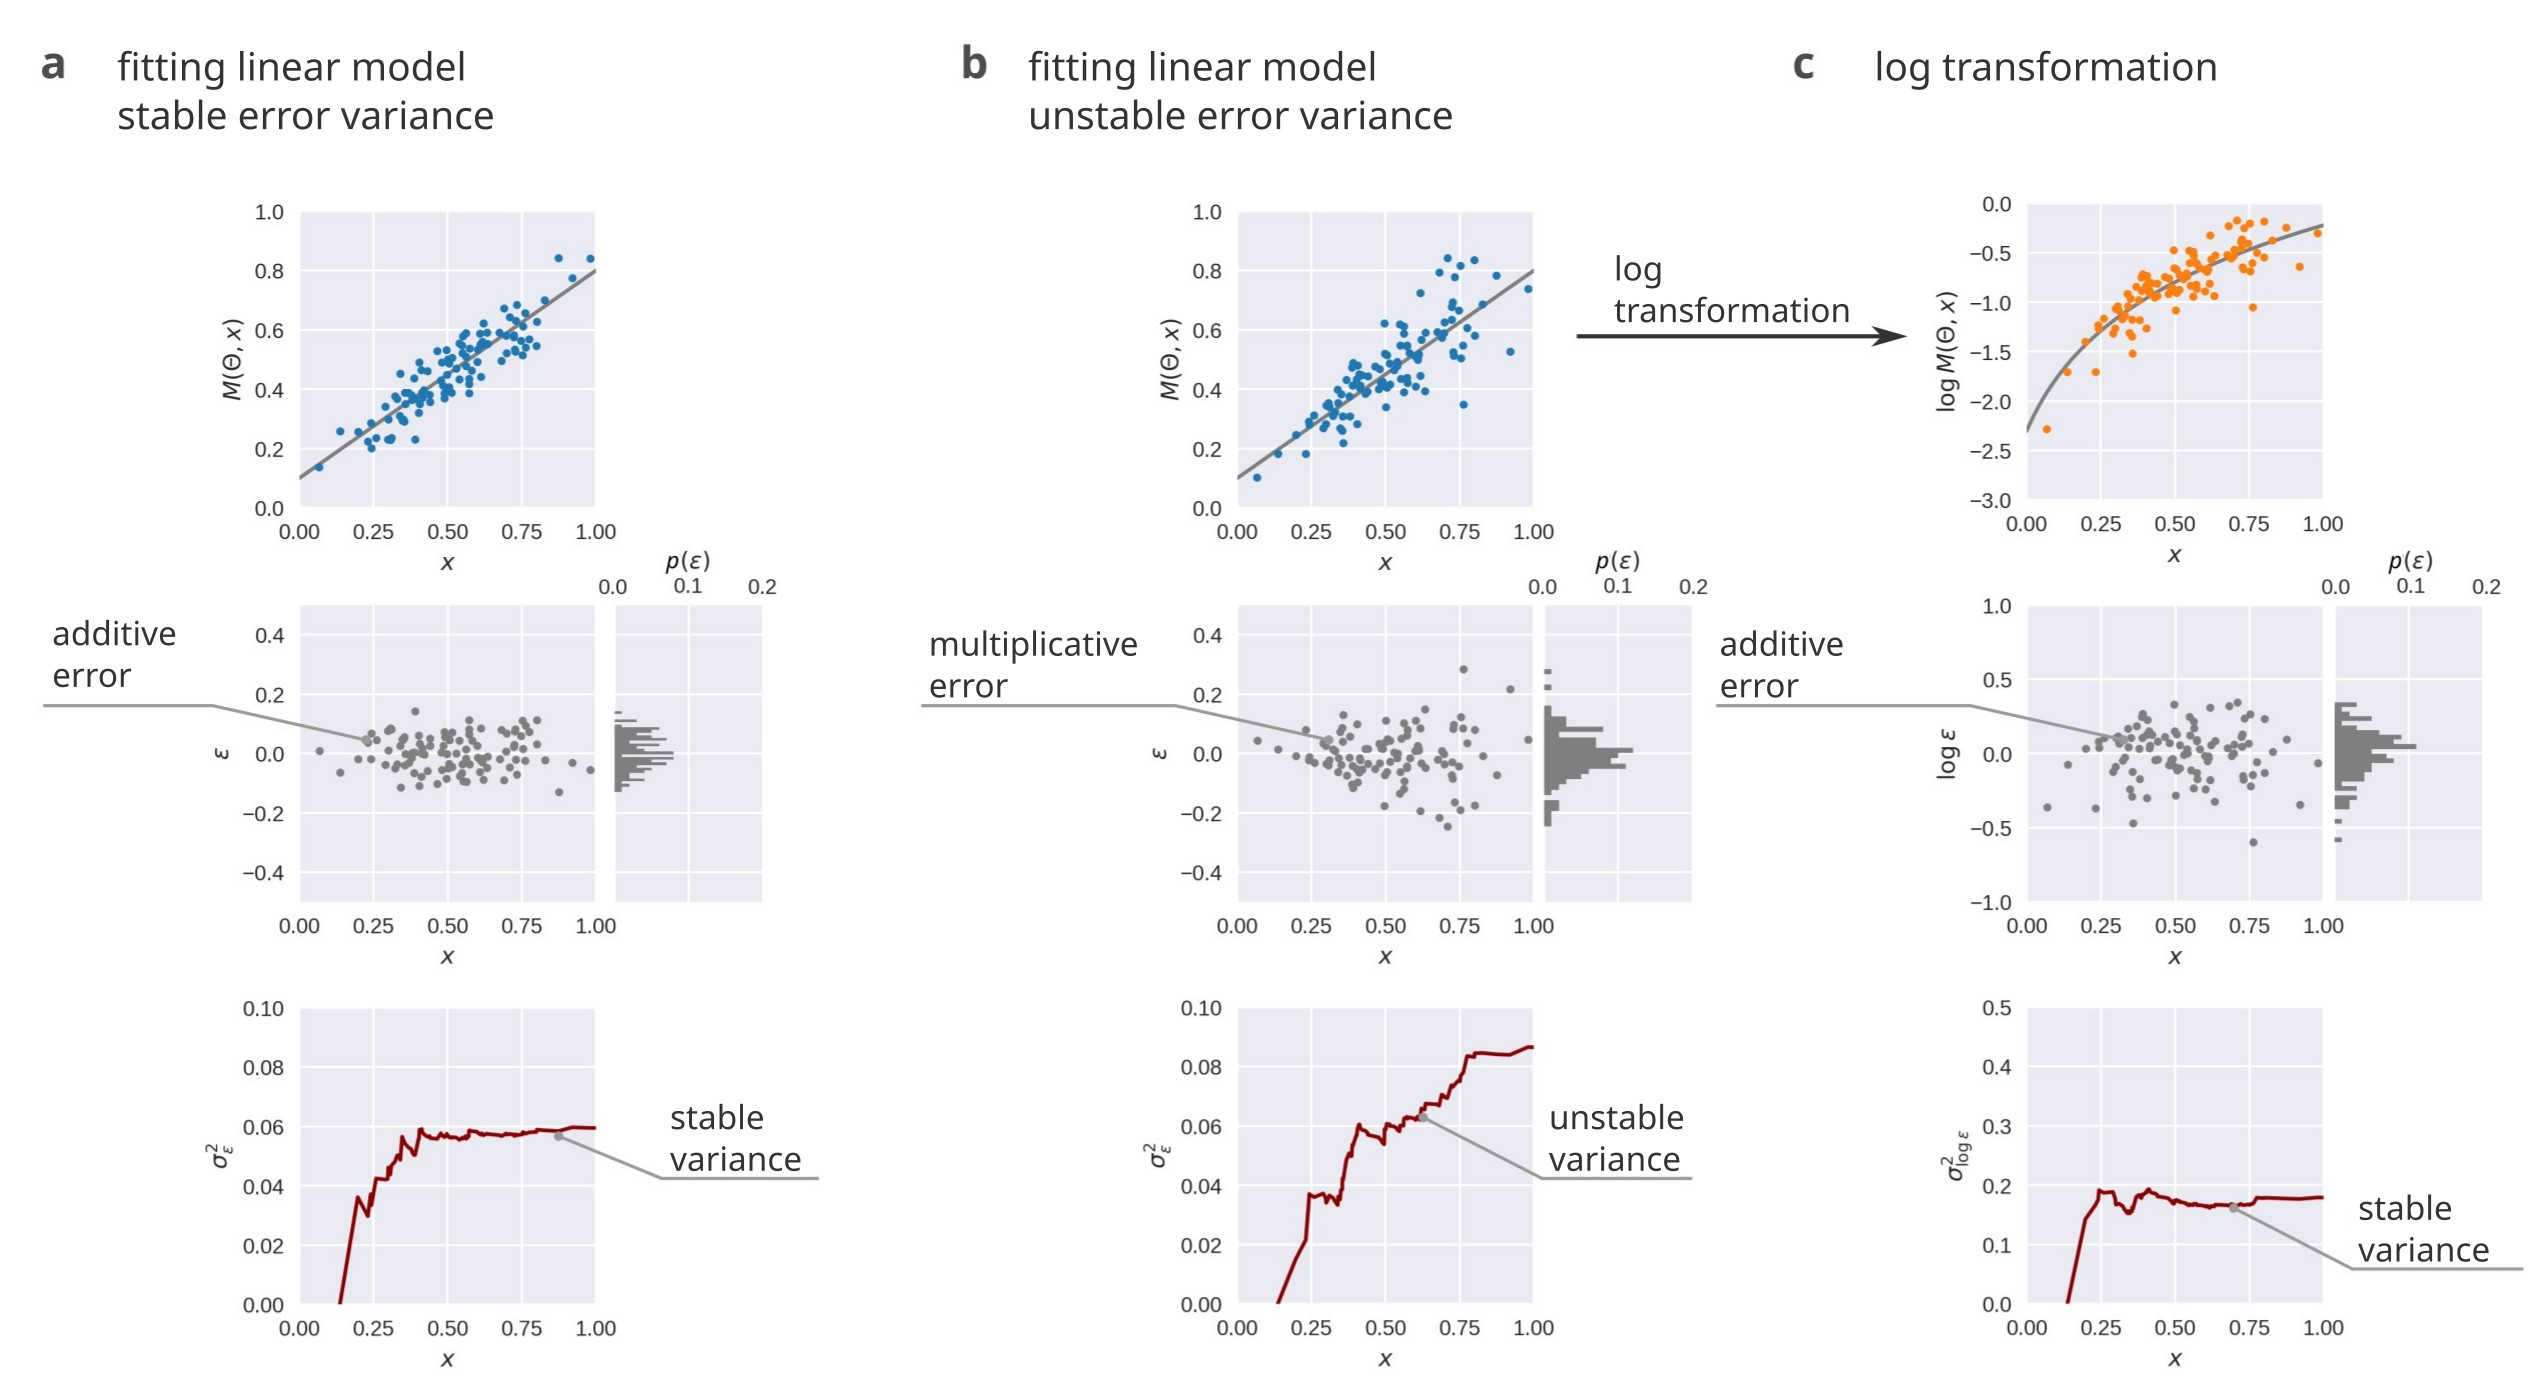
\includegraphics[width=0.95\linewidth]{fig_var_transform_en.jpg}		
	\caption[Additive error and multiplicative error]
	{\textbf{---\;Additive error and multiplicative error in the fitting of a linear \gls{model}.}
        \;\textbf{a}\;---\;Additive error in a linear \gls{model}, with stable error variance (homoscedastic).\;\textbf{b}\;---\;Multiplicative error in a linear \gls{model}, with unstable error variance (heteroscedastic).\;\textbf{c}\;---\;Stabilization of the multiplicative error variance through a logarithmic transformation. The logarithm of the error is additive.
	}
\label{fig:var_transform}  % use qualitative label			
\end{figure}

\par Figures \ref{fig:bayes_s1} and \ref{fig:bayes_s2} present an illustrative example for the \gls{conditioning} process of a \gls{model}. The goal was to condition a linear \gls{model} of the type $M(x, \Theta) = c_{1}x + c_{0}$ using the available empirical evidence\footnote{The data here is synthetic, generated for the purpose of illustrating the Bayesian approach.}. Note that $\Theta=\{c_{0}, c_{1}\}$, meaning the problem consists of obtaining the \gls{posterior} distribution of the parameters $c_0$ and $c_1$. Let’s first consider the case of the initial situation (Figure \ref{fig:bayes_s1}), when the first sample of empirical data was obtained ($n=50$). Given the data, the \gls{model} $M(x, \Theta)$ was fitted using the least squares method. The exact values obtained for the parameters in the initial fit are \textit{irrelevant}, as we are interested in obtaining a probability distribution, not precise values. The initial fit of the \gls{model} only serves to estimate the dispersion of the error $\varepsilon$. By simple visual inspection, it can be seen that the distribution of the model's errors is well-symmetrical around zero with stable dispersion. Assuming that the error $\varepsilon$ follows a normal distribution with zero mean and constant variance, the Monte Carlo method was applied with a thousand resamplings, which were done by approximating the population variance by the sample variance (i.e., $\sigma^2_\varepsilon \approx s^2_\varepsilon$). In each simulation, new fits for the \gls{model} were performed, allowing the estimation of the uncertainty bands for the \gls{model} $M(x, \Theta)$. Finally, the \gls{likelihood} distribution $P(E | H)$ of the parameters $c_0$ and $c_1$ was estimated from the histogram of the list of a thousand statistically equivalent values generated by the simulations. Since the prior distribution $P(H)$ was uniform, the posterior distribution pattern $P(H | E)$ was completely influenced by the \gls{likelihood}. Now let’s consider the second stage (Figure \ref{fig:bayes_s2}), when a new sample of empirical data was introduced ($n=50$). In this stage, the new data was mixed with the old, and the same procedure was followed: a \gls{model} was fitted to the data, and new error $\varepsilon$ simulations were conducted by approximating its population variance with its sample variance. The exception was that the prior distribution is now the posterior distribution obtained in the initial situation. With this, the arrival of new empirical observations can both \textit{reinforce} or \textit{weaken} the previously obtained \gls{grau-convic} for the parameters $c_0$ and $c_1$. In the illustrated case, it is clear that the new observations slightly weakened the \gls{grau-convic} for parameter $c_1$, slightly widening the 50\% uncertainty band obtained in the first stage and generating a bimodal posterior distribution.

\par In Equation \eqref{eq:bayes-model}, the embedded assumption is that the error $\varepsilon$ is \textit{linearly additive} to the \gls{model}. However, it could be \textit{multiplicative}, which would make Equation \eqref{eq:bayes-model} take the following form:
\begin{linenomath*}
\begin{equation}
\label{eq:bayes-model-multi}
    O(x, t) = M(x, t, \Theta) \cdot \varepsilon(x, t)
\end{equation}
\end{linenomath*}
This assumption makes sense when the random noise increases as the independent variable grows. In the case of rating curves, it is reasonable to expect that proportionally larger errors are present in the measurement of high flows from the water level, especially (but not only) due to greater uncertainties in the geometry and roughness of the channel section. When this occurs, the error variance is not constant but gradually increases. In this case, the variance is heteroscedastic (unstable), as opposed to homoscedastic (stable). An alternative to address this case is through \textbf{variable transformation}, converting the problem to an additive case by taking the logarithm on both sides of Equation \eqref{eq:bayes-model-multi}, since $\log(ab) = \log(a) + \log(b)$. Thus, the assumptions mentioned earlier can be evaluated over $\log(\varepsilon)$, which possibly shows stable variance. To apply the Monte Carlo method, the resampling of the error can be done directly on $\log(\varepsilon)$ and then converted back into Equation \eqref{eq:bayes-model-multi} for fitting the \gls{model} $M(x, \Theta)$ through optimization techniques. Figure \ref{fig:var_transform} illustrates this process.

\begin{simplebox}[
    float=htb,
    label={destaque_curvas_chave},
    nameref={Rating Curves}
    ]{Flow uncertainty bands from rating curves}
    \footnotesize
    % first minipage
    \begin{minipage}[t]{\linewidth}    
    \par \textbf{Flow} in rivers is almost never measured directly, as it requires a specialized technical team. It is much easier and cheaper to observe the \textbf{water level} in rivers using staff gauges. In fact, the water level of many rivers in Brazil is observed twice a day at streamflow stations of the National Hydrometeorological Network. Thus, the rare feasible flow observations are used to construct a \textbf{rating curve}, which is usually a power-type \gls{model}:
    \begin{equation*} % the equation environment. 
    		\label{eq:rating_curve}
    		Q = a \cdot (h - h_0)^b
    \end{equation*}
    Where $Q$ is the flow in $m^{3}/s$; $h$ is the observed level, and; $h_0$, $a$, and $b$ are the \gls{parameters} of the \gls{model}. This curve can then be used to estimate flow from routine level observations.
    \end{minipage}
    % second minipage
    \begin{minipage}[t]{\linewidth}
        \begin{minipage}[t]{\linewidth}
        \vspace*{5pt}
        	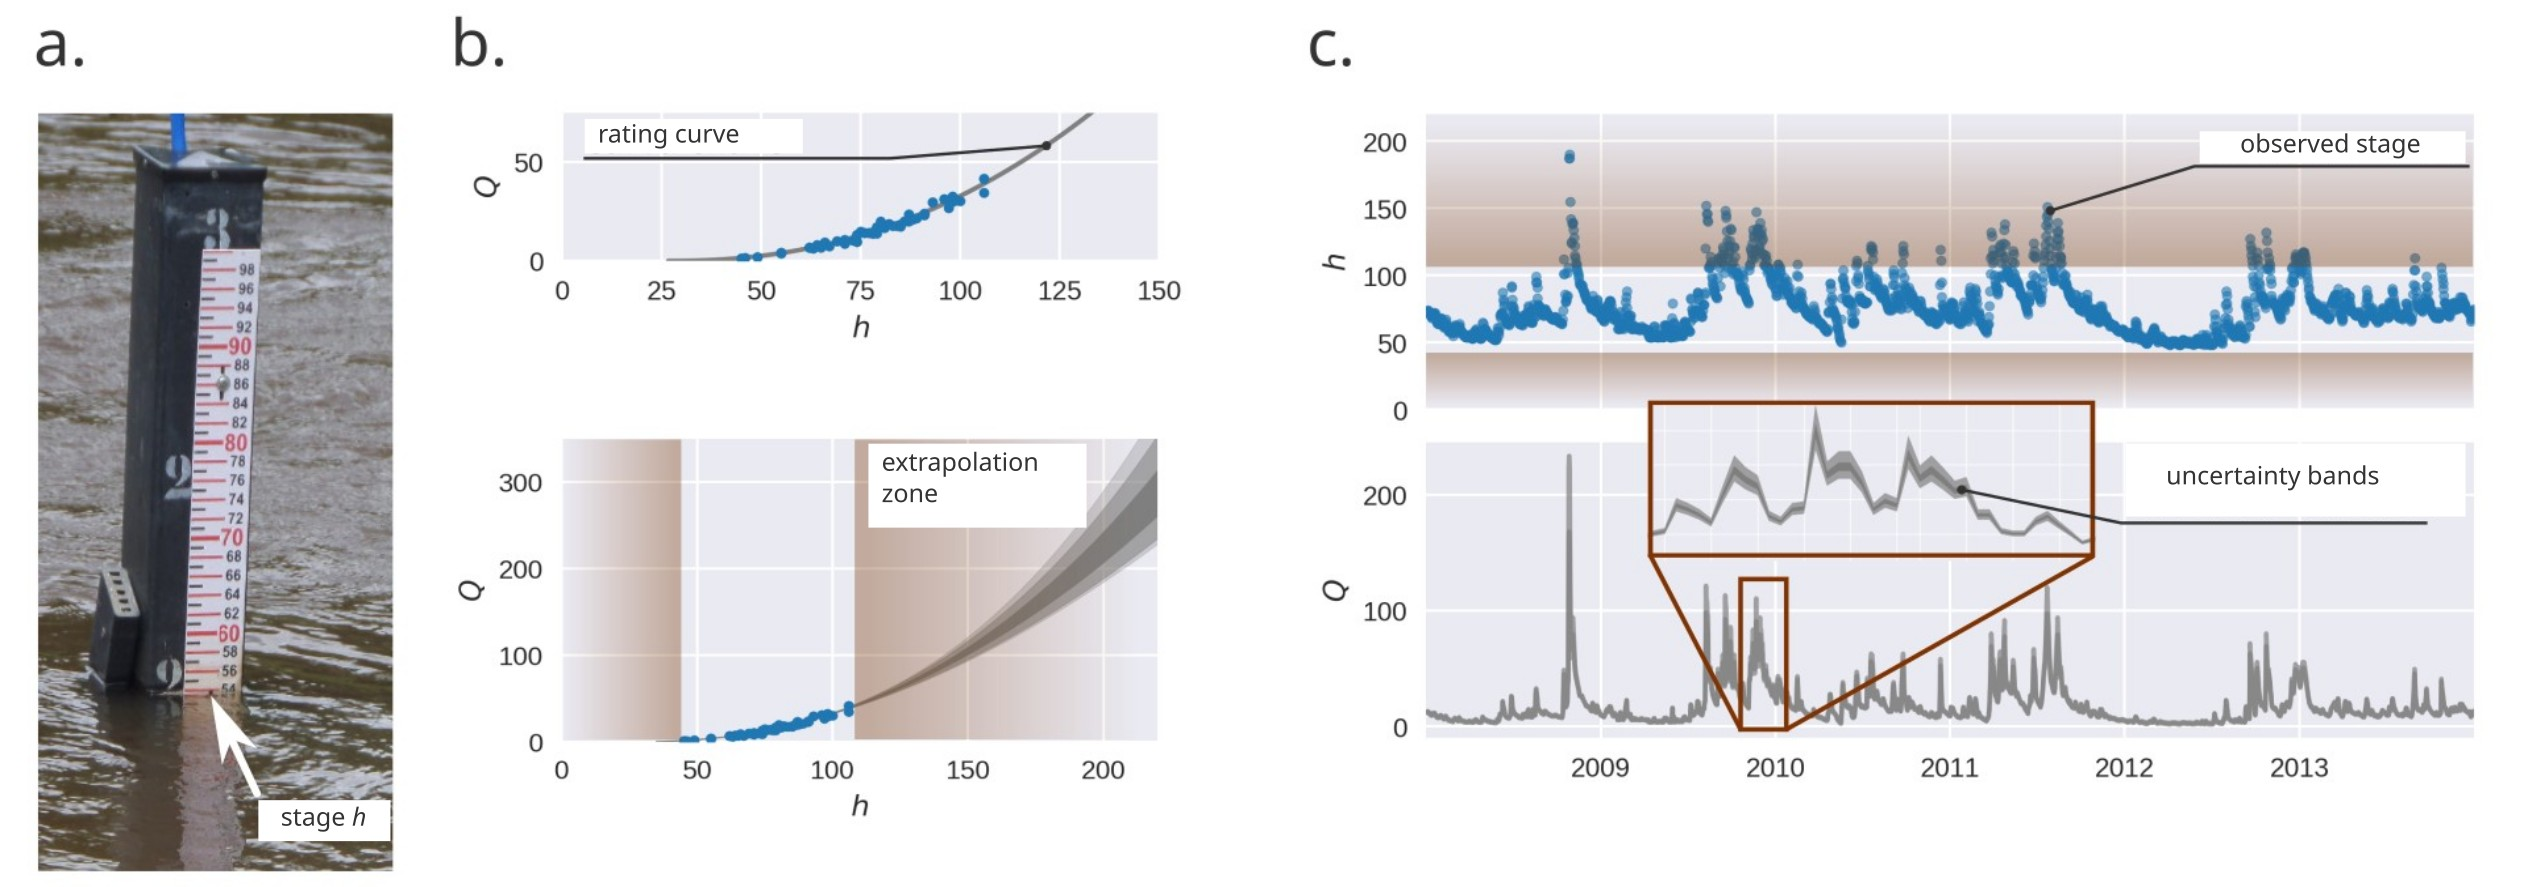
\includegraphics[width=\linewidth]{fig_ratingcurve_en.jpg}		
        	\captionof{figure}[Flow uncertainty bands from rating curves]{
                \textbf{---\;Flow uncertainty bands from rating curves.}\;\textbf{a}\;---\;Water level observation $h$ on a staff gauge.\;\textbf{b}\;---\;Fitting a power-type \gls{model} and estimating uncertainty through error resampling methods.\;\textbf{c}\;---\;Historical series of water level and flow uncertainty bands.
        	}
            \label{fig:rating-curve}  % use qualitative label	
        \vspace*{5pt}
    \end{minipage}
    % next
    \end{minipage}
    \begin{minipage}[t]{\linewidth}
    \par As illustrated in Figure \ref{fig:rating-curve}, the confirmation of this \gls{model} based on water level and flow evidence begins by fitting the \gls{parameters} to the available data using optimization techniques. The behavior of random error can then be evaluated. If the error variance is stable, statistically equivalent resamplings of the data (Monte Carlo simulations) can be performed. Thus, the uncertainty bands of the \gls{rating-curve} reflect the uncertainty in the flow estimates in the historical series. In the presented example, \textbf{extrapolation zones} can be observed at the extremes, where the uncertainty expands disproportionately. This is expected, as extreme flow events are rare or difficult to measure. On the other hand, capturing a few extreme events can drastically reduce the uncertainty in these zones.
    \par An interesting approach in this context is presented by Thomas Morlot and colleagues, who highlight that in addition to statistical uncertainties, rating curves exhibit temporal dependency associated with changes in the river section morphology \cite{Morlot2014}. Other complexities also exist, such as hydraulic hysteresis, which can manifest under different flow regimes.
    \end{minipage}
\label{box:rating-curve}
\normalsize
\end{simplebox}


\section{Rejection of theories} \label{sec:epis:popper}

\par Despite the success of \gls{empiricism} as the hegemonic current in the Philosophy of Science during modernity, the remarkable changes in Physics in the 20th century gave another chance to \gls{rationalism}, that is, the deductive approach to the \gls{problem-just}. The impact of Albert Einstein's (1879-1955) work is a good example of this historical moment. In this case, Einstein revolutionized Physics with what he called \textit{thought experiments}. If theories are products of empirical experience, as empiricists claim, Einstein would never have written his first papers, since at the time he worked at a patent office and had no access to laboratories or other resources to collect empirical data. On the contrary, it was other scientists who, through observations and experiments, supported Einstein's \gls{teoria} \textit{a posteriori}, that is, \textit{after} his ideas were already published. Something was definitely wrong with the empiricist theory justification current.

\par The exponent of this new rationalist movement was the philosopher Karl Popper (1902-1994), especially with his work \textit{The Logic of Scientific Discovery}. He introduced the current now known as \textbf{\gls{critical-rationalism}}. On one hand, Popper was aware of the seriousness of the \gls{problem-indu}, which remained (and still remains) unsolved since its formulation by Hume – for him, inductive \gls{empiricism} clearly could not be sustained. On the other hand, the philosophical currents of his time, called Conventionalists, also did not appeal to him, even though they represented deductive approaches to theory justification. In this sense, Popper concluded that the great epistemic power of empirical evidence is to justify, by the deductive method, the \textit{falsity} of a \gls{teoria}. In other words, it is through \textbf{rejection}\footnote{Here, the terms \textit{rejection}, \textit{refutation}, and \textit{falsification} are used interchangeably.} of theories by evidence that true knowledge is obtained.

\par A simple example conveys the strength of this argument.

\par Consider the universal statement that \say{\textit{all swans are white}}. To definitively establish the truth of this statement by the inductive method, it would be necessary to observe all the swans that exist in the universe, including swans in the past and future, which is obviously impossible in practice. On the other hand, it only takes seeing a \textit{single black swan} (or any other color) in time and space to definitively refute the \gls{teoria} that all swans are white. After all, if the singular statement \say{\textit{a certain swan is black}} is true (because it was empirically verified), then we deduce that the universal statement \say{\textit{all swans are white}} is false:
\begin{linenomath*}
    \begin{align*}
        S_1 \implies S_2 & \quad \textnormal{if all swans are white, then a certain swan is white} \\
        \neg S_2 & \quad \textnormal{a certain swan is \textbf{not} white}\\
        \therefore\;\neg S_1 & \quad \textnormal{therefore, not all swans are white}
    \end{align*}
\end{linenomath*}
This mode of deductive logic, involving negation, is called \textit{modus tollens}, in contrast to \textit{modus ponens}, which involves positive affirmation. What Popper demonstrates is that there is a fundamental asymmetry between these two modes of logic when we want to deduce universal statements from singular statements (make generalizations from specific observations), with \textit{modus tollens} being the only way to obtain secure knowledge (in this case, the falsity of a universal statement). Hence, observations and empirical experiences are important for refuting theories, not for confirming them. As long as a \gls{teoria} survives rigorous empirical tests, it is said that the \gls{teoria} is \textit{corroborated} by empirical evidence – but never confirmed.

\par Armed with this argument, Popper turns to what he calls the \textbf{\gls{problem-demarc}}, initially raised by Kant: the difficulty of distinguishing whether a \gls{teoria} is \textit{scientific} or merely \textit{metaphysical}, based solely on abstractions. Unlike empiricists, who claim that experience is the origin of all knowledge, for Popper the origin of where theories arise is irrelevant. As long as they are logically consistent, they can emerge either from some motivating empirical observation (like the example of white swans) or from creative intuition (such as Einstein's thought experiments). What matters is the \gls{teoria}’s ability to not survive the tests of empirical experience, that is, its ability to be rejected. This ability, called \textbf{\gls{falseabilidade}}, is the \textit{demarcation criterion} that categorizes a \gls{teoria} as scientific. In summary, from the perspective of \gls{critical-rationalism}, a scientific \gls{teoria} must be falsifiable. Here, it is important to emphasize that \textit{being falsifiable} does not mean \textit{being false}. Being falsifiable means that the structure of the \gls{teoria} allows for observations to be used to demonstrate its potential falsity. If \textit{in principle} it is impossible to prove that a \gls{teoria} is false through observations or experiments, then that \gls{teoria} is not scientific. This generally implies that scientific theories must be precise enough to produce observable predictions. In Einstein's case, his \gls{teoria} was precise and made observable predictions that were, in Popper's jargon, \textit{corroborated} by other scientists (but could have been perfectly refuted). A more intuitive example of a non-falsifiable \gls{teoria} is the Multiverse \gls{teoria}, a cosmological \gls{teoria} that postulates the existence of Universes parallel to the one we inhabit. As enticing as it may be to \textit{explain} some cosmological mysteries, this \gls{teoria} is not scientific because it does not allow for any \textit{test} with empirical observations – in principle, there is no way to observe beyond our own Universe. In Popper's words:

\begin{adjustwidth}{100pt}{0pt}
\medskip
\small (...) a \gls{teoria} is something the mind attempts to prescribe to nature; something nature often does not allow to be prescribed to her; a \gls{hipotese} we attempt to impose on nature, but which can be contradicted by her -- Karl Popper \cite{popper2013dois}.
\medskip
\end{adjustwidth}

\par Once \gls{falseabilidade} is designated as the demarcation criterion for scientific theories, Popper moves on to the so-called \textbf{problem of simplicity}. This epistemological problem consists of the difficulty in explaining why simpler theories should be preferred over more complex ones (also known as \textit{Occam's Razor}). For example, consider a series of point observations of a given phenomenon plotted in a \gls{system} of coordinates. If there is a theoretical law that describes this phenomenon, this law will be a curve connecting all the observed points. However, for a finite number of points, it is always possible to fit an infinite number of curves using various mathematical formulas. If a straight line provides a good fit, so can the asymptotic part of a hyperbola. As we saw in the previous section, while Bayesian empiricists have methods to update the \gls{grau-convic} in the fit of a given curve as new observations are collected, they have nothing to say about the justification for \textit{choosing that curve in the first place}, except for its supposed \textit{simplicity}. This is indeed a confusing problem, as it depends on what we mean by simplicity. For some, it means an aesthetic aspect, something related to mathematical elegance – like the fact that circular orbits for planets seem more beautiful than elliptical orbits. For others, it means a pragmatic aspect, something related to time and resource economy – a simpler method for solving a task should be preferred over a more intricate one. The statistician George Box (1919-2013), for instance, advocates for what he calls the \textbf{principle of parsimony} in mathematical models based on purely practical criteria, such as cognitive load, better precision, and objectivity \cite{Box1979}.

\par In view of this, Popper removes any aesthetic or pragmatic aspect, equating the simplicity of a \gls{teoria} with its \textbf{degree of \gls{falseabilidade}}: the simpler it is, the more falsifiable. This logically solves the problem of simplicity, because, in his words:

\begin{adjustwidth}{100pt}{0pt}
\medskip
\small Simple statements (...) tell us more because they contain greater empirical content and are susceptible to more rigorous testing -- Karl Popper \cite{popper2004logica}.
\medskip
\end{adjustwidth}

\noindent In other words, as long as a simpler, more \textit{restrictive} \gls{teoria} survives empirical tests, it makes no logical sense to adopt a less simple, more \textit{flexible} \gls{teoria}. This becomes clearer in mathematical terms, since the number of \gls{parameters} in a curve is inversely associated with its degree of \gls{falseabilidade}. Consider a curve with three \gls{parameters}, such as a second-degree polynomial (a parabola): $f(x) = c_{2}x^{2} + c_{1}x + c_{0}$. This curve is much more flexible for fitting data than a curve with two \gls{parameters}, such as a first-degree polynomial (a straight line): $g(x) = c_{1}x + c_{0}$. After all, if we make the quadratic parameter $c_{2}$ small enough, we can fit the data equally well with the straight line $g(x)$ without falsifying the \gls{teoria} that the studied phenomenon is described by the parabola $f(x)$, because $\lim_{c_{2}\to0} f(x) = g(x)$. The same logic applies to circular and elliptical orbits: the \gls{teoria} of the circle, being a specific case of an ellipse, should be rejected before the \gls{teoria} of the ellipse not for its aesthetics, but for its ease of being demonstrated false by observed evidence.
% figure
\begin{figure}[t!] % place figure in the page
	\centering				
	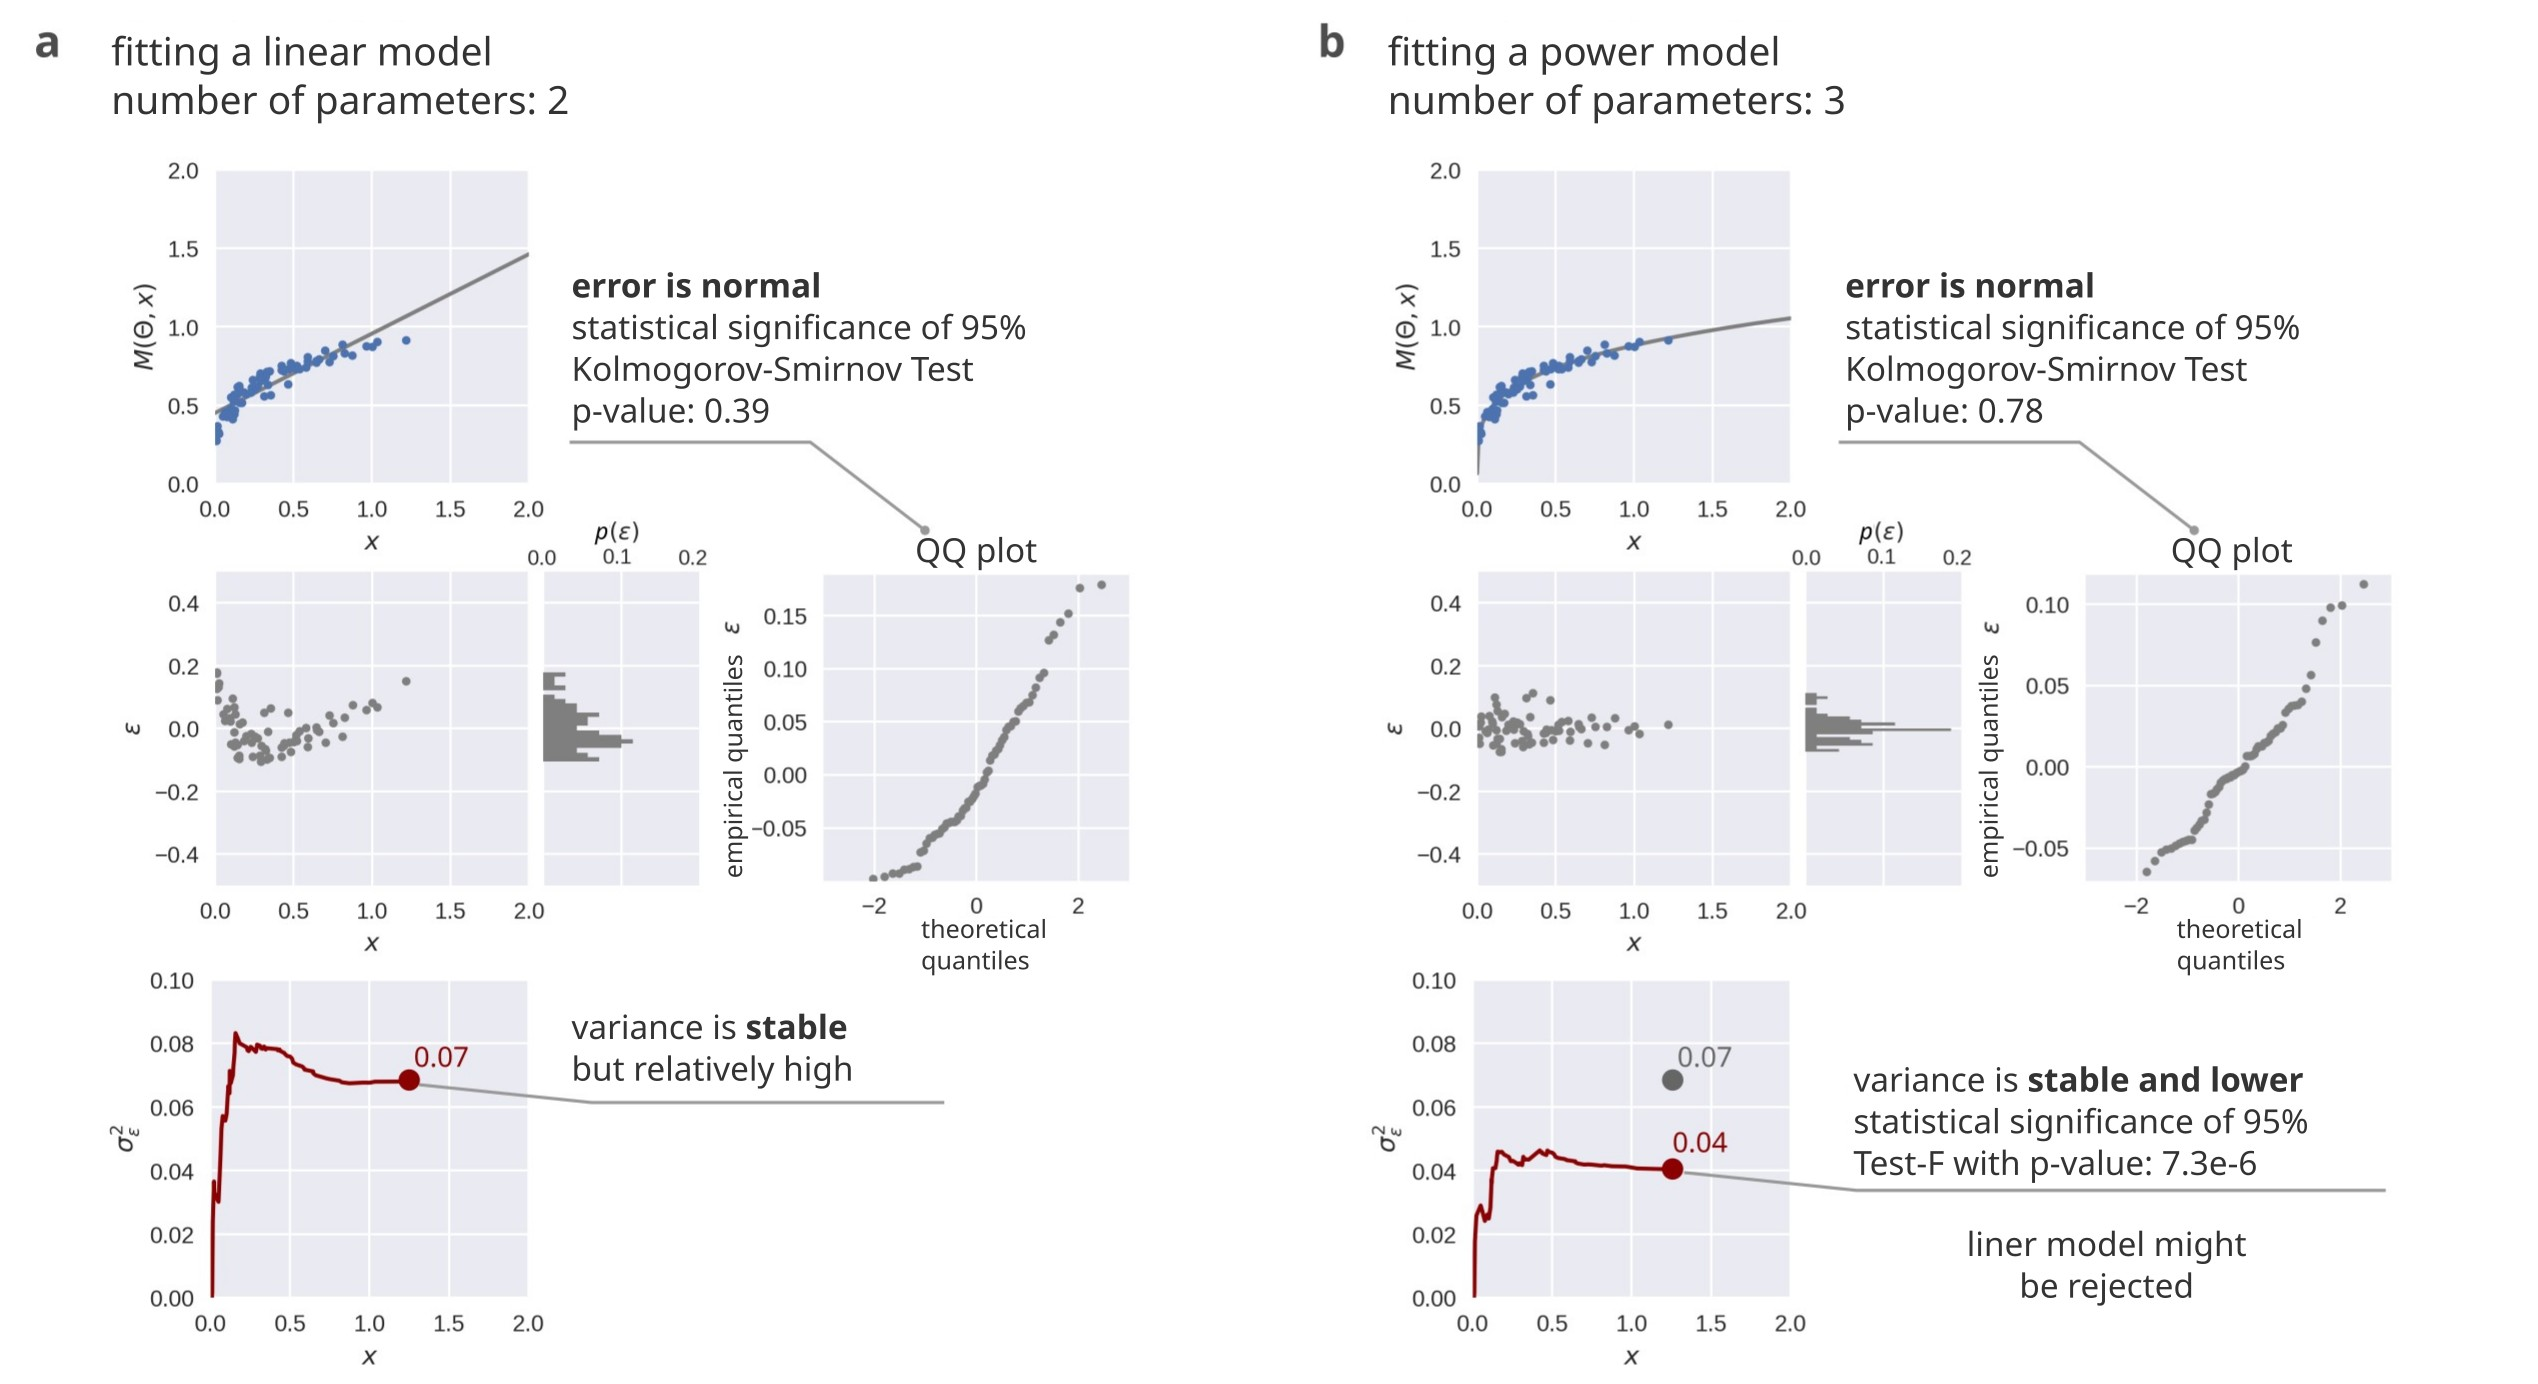
\includegraphics[width=0.95\linewidth]{fig_rejection_en.jpg}		
	\caption[Rejection criteria for model selection]
	{\textbf{---\;Rejection criteria for model selection.}
        \;\textbf{a}\;---\;Fit of a linear \gls{model} of the type $M(x, \Theta) = c_{1}x + c_{0}$. \;\textbf{b}\;---\;Fit of a power \gls{model} of the type $M(x, \Theta) = c_{1}x^{k} + c_{0}$. Both models are fitted to the same set of observed data. Both fits satisfy the assumptions of normal error and stable variance (homoscedasticity). Only by the principle of parsimony (simplicity), the linear \gls{model} should be preferred as it has fewer \gls{parameters}. But the power \gls{model} shows significantly lower error variance with 95\% statistical significance. This could be a rejection criterion for the linear \gls{model}. 
	}
\label{fig:rejection}  % use qualitative label			
\end{figure}

\par The concept of simplicity in Popper makes logical sense, but it doesn't exactly answer how to proceed when faced with observed evidence that presents random noise. In practice, it is impossible to obtain data that perfectly adheres to a mathematical relationship based on some theoretical principle, such as a linear, quadratic, or power function. Before proceeding, it is important to differentiate a \gls{teoria} from a \textbf{\gls{model-stats}}. Theories establish mathematically precise models about specific phenomena. Statistical models, on the other hand, are a very specific type of \gls{teoria} that precisely define \textit{the mathematical pattern of a dataset}, without theoretical links to the underlying phenomena\footnote{An intuitive example of this difference is to consider a population of, say, a thousand triangles with random sizes. If we look at the data for perimeter and area, we can easily create a \gls{model-stats} between these two variables: large perimeters are generally accompanied by large areas. But this is not a theoretical law about triangles, as some very acute triangles have large perimeters and small areas. The mathematical \gls{teoria} is that the area of a triangle is its base times height divided by two -- the perimeter is only partially and indirectly related.}. In the case of theories, the open question in Popper's rationalist approach is when anomalies in the data should be taken seriously enough to reject a simple \gls{teoria} in favor of a more complex one. That is, how much should the data deviate from the proposed \gls{model} for the \gls{teoria} to be considered falsified by the evidence? This question inevitably introduces a decision, which is the prior definition of a \textbf{rejection criterion}. The decision on the rejection criterion needs to be \textit{before} the evaluation of the \gls{teoria} (\textit{a priori}) because if it is \textit{after}, nothing prevents the \gls{teoria} from never being rejected -- one just needs to establish a criterion that is known to be lenient. Popper himself criticizes theories that, in the face of clearly falsifying evidence, resort to subterfuges and \textit{ad hoc} explanations to try to survive. This dilemma becomes evident in the case of the premises mentioned in Section \ref{sec:epis:bayes} regarding the \gls{model-stats} of random noise: zero mean, constant variance, independence over time, and normal distribution. For example, one can evaluate the premise of normality of the error $\varepsilon$ using a Quantile-Quantile plot or hypothesis tests, such as the Kolmogorov–Smirnov test. In the case of the Quantile-Quantile plot, the interpretation is purely visual. If the plot deviates significantly from a straight line, the premise should be rejected. In the case of the hypothesis test, the confidence level for the null hypothesis is defined \textit{a priori}. If the desired confidence level is set at 95\%, a p-value less than or equal to 0.05 indicates that the probability of normality given the considered data is less than 5\%, and the premise should be rejected. Is there a logical justification for the 95\% level? There is none. Another example, illustrated in Figure \ref{fig:rejection}, is when all the premises about the residuals are satisfied by both a simple \gls{model} and a complex \gls{model}, but the complex \gls{model} is more \textit{accurate} than the simple \gls{model}, meaning the error dispersion is \textit{less}. How much should the dispersion be less to reject the simpler \gls{model}? Again, one could apply a hypothesis test for equal variances, the F-Test, and obtain an answer for a previously defined confidence level. If the variances are statistically significantly different, the simpler \gls{model} should be rejected. One way or another, there is subjectivity involved in rejection, as criteria or thresholds defined \textit{a priori} are necessary.

\section{Paradigm shifts} \label{sec:epis:kuhn}

\par In the Philosophy of Science, there is an important distinction between \textbf{\gls{contexto-justificacao}} and \textbf{\gls{contexto-descoberta}}. The first context addresses the epistemological problem of how to justify the truth of a \gls{teoria}. The second context investigates the historical and sociological problem of how progress occurs in Science – if indeed progress exists. The different philosophical currents mentioned in the previous sections fit into the first context, as they provide solutions to the epistemological problem of justification. In one way or another, they assign an important role to empirical evidence. For Bayesian empiricists, evidence would be used inductively to confirm the \gls{grau-convic} in a \gls{teoria} based on the mathematics of probabilities. For critical rationalists, evidence would be essential to falsify theories through deductive logic, leaving theories in an eternal provisional state – they would be corroborated but never confirmed. \textit{Confirmation} and \textit{rejection}, thus, form a somewhat paradoxical dichotomy, as both make sense in the practice of Science, but contradict each other. This paradox is resolved by the perspective of the \gls{contexto-descoberta}. In his work \textit{The Structure of Scientific Revolutions}, Thomas Kuhn (1922-1996) provides substantial contributions in this regard.

\par As a historian, Kuhn warns that Science does not exist in a vacuum: rather, it is composed of a \textit{community} of human beings who interact over History, across successive generations, within a larger society. The existence of the \textbf{\gls{comunidade-cientifica}} implies that one must consider not only the History of Science but also the Sociology of Science to understand the \gls{contexto-descoberta}. This community is obviously not a single block, but a social network of smaller communities across different disciplines and fields of knowledge. In this light, Kuhn proposes that the dynamics of a given \gls{comunidade-cientifica} produce a cyclical historical pattern, structured into three interconnected phases: the period of \textbf{\gls{ciencia-normal}}, the period of \textbf{crisis}, and the period of \textbf{revolution}. Thus, the confirmation and falsification of theories predominately occur at different stages of this historical pattern, with confirmation being a dominant process in the \gls{ciencia-normal} period and rejection being an essential characteristic of the crisis period. However, the most important process for change in Science, occurring during the revolutionary period, is the \textbf{competition} between theories. In his words:

\begin{adjustwidth}{100pt}{0pt}
\medskip
\small (...) the competition between segments of the \gls{comunidade-cientifica} is the only historical process that actually results in the rejection of an previously acceptable \gls{teoria} or the adoption of another. -- Thomas Kuhn \cite{kuhn2012structure}.
\medskip
\end{adjustwidth}

\noindent This process is inevitably intergenerational, as new members of the community need to be reeducated to think within a new worldview. To illustrate this point, Kuhn cites a striking excerpt from the autobiography of physicist Max Planck (1858-1947):

\begin{adjustwidth}{100pt}{0pt}
\medskip
\small (...) a new scientific truth does not triumph by convincing its opponents and making them see the light, but rather because its opponents eventually die, and a new generation grows up familiar with it. -- Max Planck \textit{apud} Thomas Kuhn \cite{kuhn2012structure}.
\medskip
\end{adjustwidth}

\par A key idea for Kuhn is that a \gls{comunidade-cientifica} shares a common \textbf{\gls{paradigma}}. By \gls{paradigma}, he refers to a set of exemplary solutions for research problems, meaning a \gls{system} of theories, instruments, and auxiliary practices that effectively solve certain widely accepted problems and are \textit{promising} for addressing mysterious and controversial issues with great competitive appeal. This competitive appeal is crucial, as the attraction of segments of the community around a \gls{paradigma} creates a positive \gls{feedback}: the more segments adopt the \gls{paradigma}, the more new segments become convinced that they need to adopt it as well, under the penalty of falling behind. The \gls{comunidade-cientifica} in the normal period thus operates on both theoretical and applied fronts to reaffirm and articulate the hegemonic \gls{paradigma}. Scientific research during this period is not explicitly aimed at discovering unexpected novelties; instead, the success of normal research is defined precisely by not encountering any surprises. A successful research effort typically confirms what the prevailing \gls{paradigma} has already promised by providing a more refined detailing or by expanding the range of applications (for example, through the invention of new technologies). Like a jigsaw puzzle, in \gls{ciencia-normal}, it is presumed in advance what the complete picture that the pieces form looks like – the only challenge is to fit the pieces together. Here, the sense arises that Science is a \textit{cumulative} endeavor: each new member introduced into the \gls{comunidade-cientifica} would have the humble mission of laying another small brick in the grand \say{edifice of human knowledge}. In Kuhn's view, this impression of accumulation, besides being misleading in the larger context, is reinforced by the widespread use of textbooks in training new researchers. These textbooks serve as vehicles for the perpetuation of the hegemonic \gls{paradigma} because, when they are not simply written in an anti-historical manner, they distort History to make it appear as a linear and inevitable process leading to current theories.

\par Kuhn argues, with various examples from the History of Science, that the pieces of the puzzle studied by \gls{ciencia-normal} eventually do not fit together. While knowledge accumulates during the normal period, empirical and theoretical \textbf{anomalies} also accumulate. Typically avoided or ignored, at some point these anomalies begin to cause widespread discomfort within the \gls{comunidade-cientifica}, leading it into the crisis period. The most detailed example of crisis provided by Kuhn is that of geocentrism, but he also offers examples in chemistry, mechanics, and electromagnetism. From this perspective, history shows that some crises develop slowly, as in chemistry, while others are sudden, like the one caused by Einstein in Physics. A \gls{comunidade-cientifica} in crisis exhibits various symptoms, such as discord, discontent, philosophical debates, and, most importantly, the widespread proliferation of candidate theories to explain the anomalies.

\par The only way out of the crisis is the revolution brought about by the proposal of a \gls{paradigma} that is irresistible to the \gls{comunidade-cientifica}. As previously noted, the new \gls{paradigma} must be effective in solving already known problems and make enticing promises for solving open issues. The new ideas must, in some way, offer a \textbf{retrocompatibility} with the old ideals without being contaminated by the problems embedded in the fundamental principles of the old ideas. Scientific revolutions, therefore, are episodes in which the supposed edifice of knowledge is demolished so that a new structure can be erected on a new foundation, with a new blueprint. During this revolutionary period, which typically lasts a generation, the \gls{comunidade-cientifica} migrates en masse to the new \gls{paradigma}. New textbooks are then written, and a new historical cycle of \gls{ciencia-normal} is established. An important aspect of this process is that, for Kuhn, a new \gls{paradigma} is so fundamentally different from the old one that they are \textit{incommensurable}: intellectual communication between them is extremely precarious, as they represent different worldviews. Typical examples of \textbf{\gls{incomensu-theory}} occur with the concepts of mass, space, and time in Newtonian physics and in Einstein's physics. Despite having the same name and symbol, these concepts have distinct meanings under the different paradigms, with distinct theoretical implications\footnote{In the Newtonian \gls{paradigma}, gravity is an attractive force related to mass that acts instantaneously at a distance. In the Einsteinian \gls{paradigma}, gravity is not a force but a \textit{consequence} of the distortion of space itself, implying the existence of gravitational waves. For Kuhn, Einstein does not merely extrapolate the limits of Newton: he produces a new worldview that is irreconcilable with the previous one.}. Thus, Kuhn brings forth a troubling conclusion: that there is \textit{no absolute progress} in Science towards the truth about reality, only \textit{relative} to what we are concerned with explaining. More than that, with his thesis, Kuhn highlights the depth of the social dynamics surrounding Science, which is often portrayed as the most rational of human endeavors\footnote{Kuhn's emphasis on the relativity of knowledge, historical contingency, and the presence of paradigms has invigorated the emergence of the philosophical current of \textbf{postmodernism}, bringing with it the notion that human knowledge is a \textbf{discourse}. Thus, postmodernists reject grand absolutist narratives and emphasize the linguistic, cultural, and especially political influences that permeate the production of knowledge.}.

\par As previously outlined, Thomas Kuhn's thesis on the \gls{contexto-descoberta} eliminates the paradox between confirmation and rejection, which are contradictory solutions in the \gls{contexto-justificacao}. However, a cautious look reveals that Kuhn's approach is essentially empiricist: he seeks to \textit{confirm} the ideas of paradigms and scientific revolutions based on examples from the History of Science, that is, based on \textit{empirical evidence}. Kuhn employs \gls{infer-indu} to justify a \gls{teoria} about the \gls{contexto-descoberta}. From the perspective of critical rationalism, no matter how well corroborated, a single counterexample would be sufficient to falsify Kuhn's \gls{teoria}. The problem is that this fact, paradoxically, \textit{resurrects the dichotomy between confirmation and falsification}. To make matters worse, if Kuhn's \gls{teoria} is scientific (i.e., falsifiable), wouldn't it itself be a \textit{paradigm} for how to explain the \gls{contexto-descoberta}? Here arises a recursive loop of self-reference. Recursion in an argument is typically an indicator of the \gls{problem-regress} mentioned earlier. This is a typical terrifying situation of being endlessly caught in circles that Philosophy provides. Karl Popper, perhaps because he was a philosopher and not a historian, seems to have foreseen these problems and pre-established that the \gls{teoria} on the scientific method cannot itself be scientific – falsifiable by evidence – but only a \gls{teoria} based on Logic.

\section{The problem of underdetermination} \label{sec:epis:under}

\par What we have seen so far fits into the broader philosophical current known as \textbf{\gls{realism-sci}}. This current essentially defends the thesis that the purpose of Science is to provide theories that are true descriptions of reality \cite{bas1980}. For example, we began this chapter by mentioning that Keith Beven classifies the philosophy of most users of hydrological models as \textit{\gls{prag-realism}}, which is the tacit understanding that models provide an approximate description of reality that can be improved with new technologies. The \gls{prag-realism}, for Beven, would be a branch of \gls{realism-sci}. The origins of \gls{realism-sci} can be traced back to the ideas of René Descartes \cite{Agazzi2017}. Here, it is important to establish that \textbf{\gls{realism}} itself consists of the conception in Metaphysics that admits the existence of an \textit{objective} reality, meaning that the world does not depend on anyone to observe it. In this sense, when a person enters a room and observes a table, it is assumed that the table was there before they entered. The table did not come into existence at the moment of observation. Objects, like tables, exist independently of subjects. This conception opposes \textbf{\gls{idealism}}, a current that considers reality strictly as a product of subjects, that is, \textit{subjective}. If we agree on the existence of a supposed object, like a table, it is because it manifests similarly in our minds, that is, \textit{intersubjectively}. Descartes flirts with \gls{idealism} when he questions his own existence in the \textit{Discourse on the Method}, particularly with the branch of solipsism—the idea that the mind of the person reading this text is the only thing that truly exists. Descartes basically points out that, although we have absolute certainty about the ideas in our minds, it is difficult to guarantee that they correspond to external reality. In his terms, \textit{\gls{likelihood} does not imply truth}. To try to resolve this problem, Descartes describes the method of doubt, which inspired the formation of the modern scientific method, contributing to the debate around the \gls{problem-just} that we have addressed so far. Ultimately, the \gls{problem-just} is inherently contaminated by the \textit{assumption that objective reality exists}, with the concept of \textbf{truth} being precisely the \textit{correspondence} between theories and reality.

\par The thesis of \gls{realism-sci} seems obvious, but defending it is not so straightforward. In fact, Bas van Fraassen \cite{bas1980} and Nancy Cartwright \cite{nancy1983} provide a profound critique, proposing a radically empiricist viewpoint known as \textbf{\gls{instrument}}\footnote{Instrumentalism is a broad and neutral term. For example, van Fraassen self-identifies his thesis as \textit{\gls{empiricism} constructivist}. Realists, on the other hand, classify \gls{instrument} as \textit{anti-realism}.} \cite{sep-constructive-empiricism}. Both argue that the objective of Science is to produce theories that exhibit \textit{empirical adequacy}—and nothing beyond that. Since empirical adequacy does not logically imply a true description of reality, the claim of \gls{realism-sci} is too ambitious in epistemological terms. This viewpoint does not deny the existence of reality (it is not an idealist current): what it denies is the ambition of obtaining a true description of reality. Theories and their models would merely be \textit{instruments} constructed by scientists to explain empirical evidence. One of the main reasons for this claim is the \textbf{\gls{problem-subdet}}, which is the difficulty of ensuring that the observed evidence determines the truth of a \gls{teoria} without there being empirically equivalent theories \cite{sep-scientific-underdet}, \cite{Tulodziecki2017}. Popper's orientation to always prefer the simplest \gls{teoria} works well only for theories that are completely falsifiable by empirical evidence. This is not the case for most theories, which almost always postulate the existence of \textit{unobservable entities} to explain phenomena that are directly observable. For example, in Physics, the existence of electrons and electromagnetic fields (unobservable) is invoked to explain the lightning and thunder of a storm (observable). This complicates matters, as no matter how we detect unobservable entities, like electromagnetic fields, indirect evidence will always be contaminated with a \textit{theoretical load} that establishes the existence of these entities in the first place. This type of theoretical approach involves a kind of reasoning that is non-deductive, called \textbf{\gls{ibe}}, or abduction. Because it is not deductive, this reasoning does not guarantee the truth of the consequent and is also subject to the \gls{problem-indu} postulated by Hume. Thus, a \gls{teoria} that instantiates unobservable entities pays the price of being underdetermined by observable empirical evidence.

\par One of the main defenses of \gls{realism-sci} consists in evoking the success of Science as evidence that scientific theories, even when instantiating unobservable entities, progress toward describing reality in an increasingly true manner \cite{saatsi2017}. From the critical rationalist perspective, although the ultimate truth about reality remains permanently shielded, the rejection of theories allows for the incremental isolation of a set of potentially true ideas. Indeed, it is undeniable that the theoretical predictions and technological applications that Science has produced in recent centuries are impressive and unprecedented in historical terms. Given all this success, it even sounds somewhat absurd to consider that modern Science does not describe reality. Although \gls{ibe} does not guarantee a logical implication, as instrumentalists correctly point out, defenders of \gls{realism-sci} argue that it would be \textit{a miracle} extremely unlikely for current theories to achieve good results for the wrong reasons. However, Donald Hoffman introduces the possibility that scientific theories describe the behavior of a \textit{cognitive interface} with remarkable empirical adequacy \cite{Hoffman2015}. He argues that cognitive systems, when subjected to natural selection, are pressured to operate through \textbf{\gls{heuristic}}. That is, those systems that condense the necessary information to make useful decisions gain a competitive advantage. The evolution of these systems results in a perceptual interface optimized for survival and reproduction, but whose probability of being equivalent to reality is \textit{precisely zero}. As an \gls{analogy}, consider the graphical interface of a computer. In this case, we can easily observe the behavior of buttons and icons to identify patterns without knowing anything about the underlying electronic mechanisms. The information from the graphical interface tells us absolutely nothing about the \textit{hardware}. For Hoffman, the truth about reality may simply have nothing to do with space, time, energy, matter, etc.—in Kantian terms, these would be the transcendental categories we use to condense and integrate perceptual information \footnote{Donald Hoffman subverts the \gls{paradigma} of material physicalism by proposing that reality is not fundamentally constituted of subatomic particles, but rather of an infinite network of interactions among conscious agents \cite{Hoffman2023}. The interactions of these agents produce cognitive interfaces that eventually instantiate self-referential ties, that is, realize a \textit{Self}, an \say{I}. This \gls{hipotese} simultaneously explains why subjective experiences exist (note that they are not predicted within material physicalism) and why \gls{realism} definitely does not hold at quantum scales (the supposedly physical properties are realized instantaneously at the moment of observation).}

\par The \gls{problem-subdet} has direct and relevant implications for users of environmental models, including hydrological models. In this context, Naomi Oreskes and colleagues point out that underdetermination occurs because various processes represented by the models are not observable \textit{in practice}, meaning that information about the modeled \gls{system} is \textit{incomplete} both in time and space \cite{Oreskes1994}. This milder version of underdetermination is also referred to as the \textbf{\gls{problem-equifinal}} \cite{Beven2006}. For example, consider the groundwater flow occurring in watersheds. It is evident that this process exists: a field expedition makes this clear by directly observing the springs of streams, the places where groundwater flows to the surface. In fact, piezometers can be installed to monitor the water table level, providing more direct evidence of this process. However, the extent and complete dynamics of these underground flows are practically impossible to monitor, being observable only in specific points. Oreskes \textit{et al.} argue that the partiality of the information renders the modeled natural systems \textit{logically open}. Unlike logically closed systems, such as algorithms and mathematical equations, they point out that it is impossible to verify or validate a logically open \gls{system} in light of \textit{extenuating circumstances} that often ensure empirically equivalent explanations, or \textit{equifinal}. This is intuitive: when we do not have complete information about some event we observe, it is natural for rival and equally valid explanations to emerge. Indeed, it is precisely for this reason that scientific experiments are designed to reduce the logical openness of the evaluated \gls{system}, that is, to lessen the influence of extenuating circumstances. Thus, models of natural systems present themselves as a \textbf{main hypothesis} that requires the assistance of \textbf{\gls{aux-hyp}} — such as \gls{parameters}, \gls{input-data}, the adopted scales, and, especially, the underlying theoretical assumptions. This gives rise to a paradox: it is precisely due to the lack of information that the application of models is sought in the first place. If the information were already completely available, it is unlikely that a \gls{model} would be relevant for decision-making. But without complete information, a \gls{model} becomes underdetermined by the available evidence—the inexorable \gls{problem-subdet} in model application.

\par For Keith Beven, recognizing the \gls{problem-subdet} in hydrological modeling brings radical consequences for the confirmation of models in light of observed evidence, specifically the need to evaluate the \textbf{total error} associated with a given hydrological \gls{model} \cite{Beven2005}. From this perspective, Equation \eqref{eq:bayes-model} would be incomplete, as the error $\varepsilon$ there represents only the random noise related to the observed evidence. It is necessary to include not only the \textbf{\gls{uncert-stats}}, resulting solely from sampling noise, but also the \gls{uncert-episteme}, which arises from the \gls{aux-hyp} necessary to address the \gls{problem-subdet} \cite{Beven2016}. Thus, the \textbf{\gls{eq-total-error}} for hydrological models takes the following form:
\begin{linenomath*}
\begin{equation}
\label{eq:total-error}
    O(x, t) + \varepsilon_{O}(x, t) + \varepsilon_{\Delta}(\Delta x,\Delta t, x, t) = M(\Theta, \Upsilon, \varepsilon_{\Upsilon}, x, t) + \varepsilon_{M}(\Theta, \Upsilon, \varepsilon_{\Upsilon}, x, t) + \varepsilon_r
\end{equation}
\end{linenomath*}
where $O(x, t)$ is the observation obtained at the independent variable $x$\footnote{In hydrological models, the independent variable is usually two-dimensional space, meaning $x$ should be replaced by $x, y$.} and at time $t$; $\varepsilon_{O}(x, t)$ is the \textbf{\gls{error-measure}} of the observation; $\varepsilon_{\Delta}(\Delta x,\Delta t, x, t)$ is the \textbf{\gls{error-commensu}} at the modeling scale $\Delta x$ and $\Delta t$; $M(\Theta, \Upsilon, \varepsilon_{\Upsilon}, x, t)$ is the prediction of the \gls{model} at $x, t$ based on the vector of \gls{parameters} $\Theta$, the vector of \gls{input-data} $\Upsilon$, and the \textbf{\gls{error-input}} $\varepsilon_{\Upsilon}$; $\varepsilon_{M}(\Theta, \Upsilon, \varepsilon_{\Upsilon}, x, t)$ is the \textbf{\gls{error-struct}}, and; $\varepsilon_r$ is the \textbf{random error} remaining. The \gls{error-commensu} $\varepsilon_{\Delta}$ results from the conversion between scales, representing the \gls{uncert-episteme} of the difference in meaning between an observation obtained at \textit{x, t} and the corresponding modeled variable at $\Delta x, \Delta t$. For example, while the observed flow of a river is instantaneous and refers to a specific section of the channel, the modeled flow integrates some time step and refers to a discrete spatial extent. The \gls{error-measure} $\varepsilon_{O}$ and the \gls{error-commensu} $\varepsilon_{\Delta}$ are kept on the left side of Equation \eqref{eq:total-error} to denote that together they constitute the \textbf{\gls{error-obs}}. The \gls{error-input} $\varepsilon_\Upsilon$ originates from the aggregation of uncertainties in both boundary conditions (such as maps of topography, soil, vegetation, etc.) and the forcing variables of the \gls{model} (such as rainfall, temperature, wind speed, etc.). In this case, the uncertainty is generally statistical, so representative samples tend to reduce its impact. However, it can also take on an epistemic nature when the input data correspond to \textbf{scenarios}, which adds a conceptual burden. Finally, the \gls{error-struct} $\varepsilon_M$ results from the \gls{uncert-episteme} of the theoretical and numerical configuration of the hydrological \gls{model}. This component is strongly influenced by the theoretical assumptions previously defined about the \gls{system} and its hydrological processes.

% figure
\begin{figure}[t!] % place figure in the page
	\centering				
	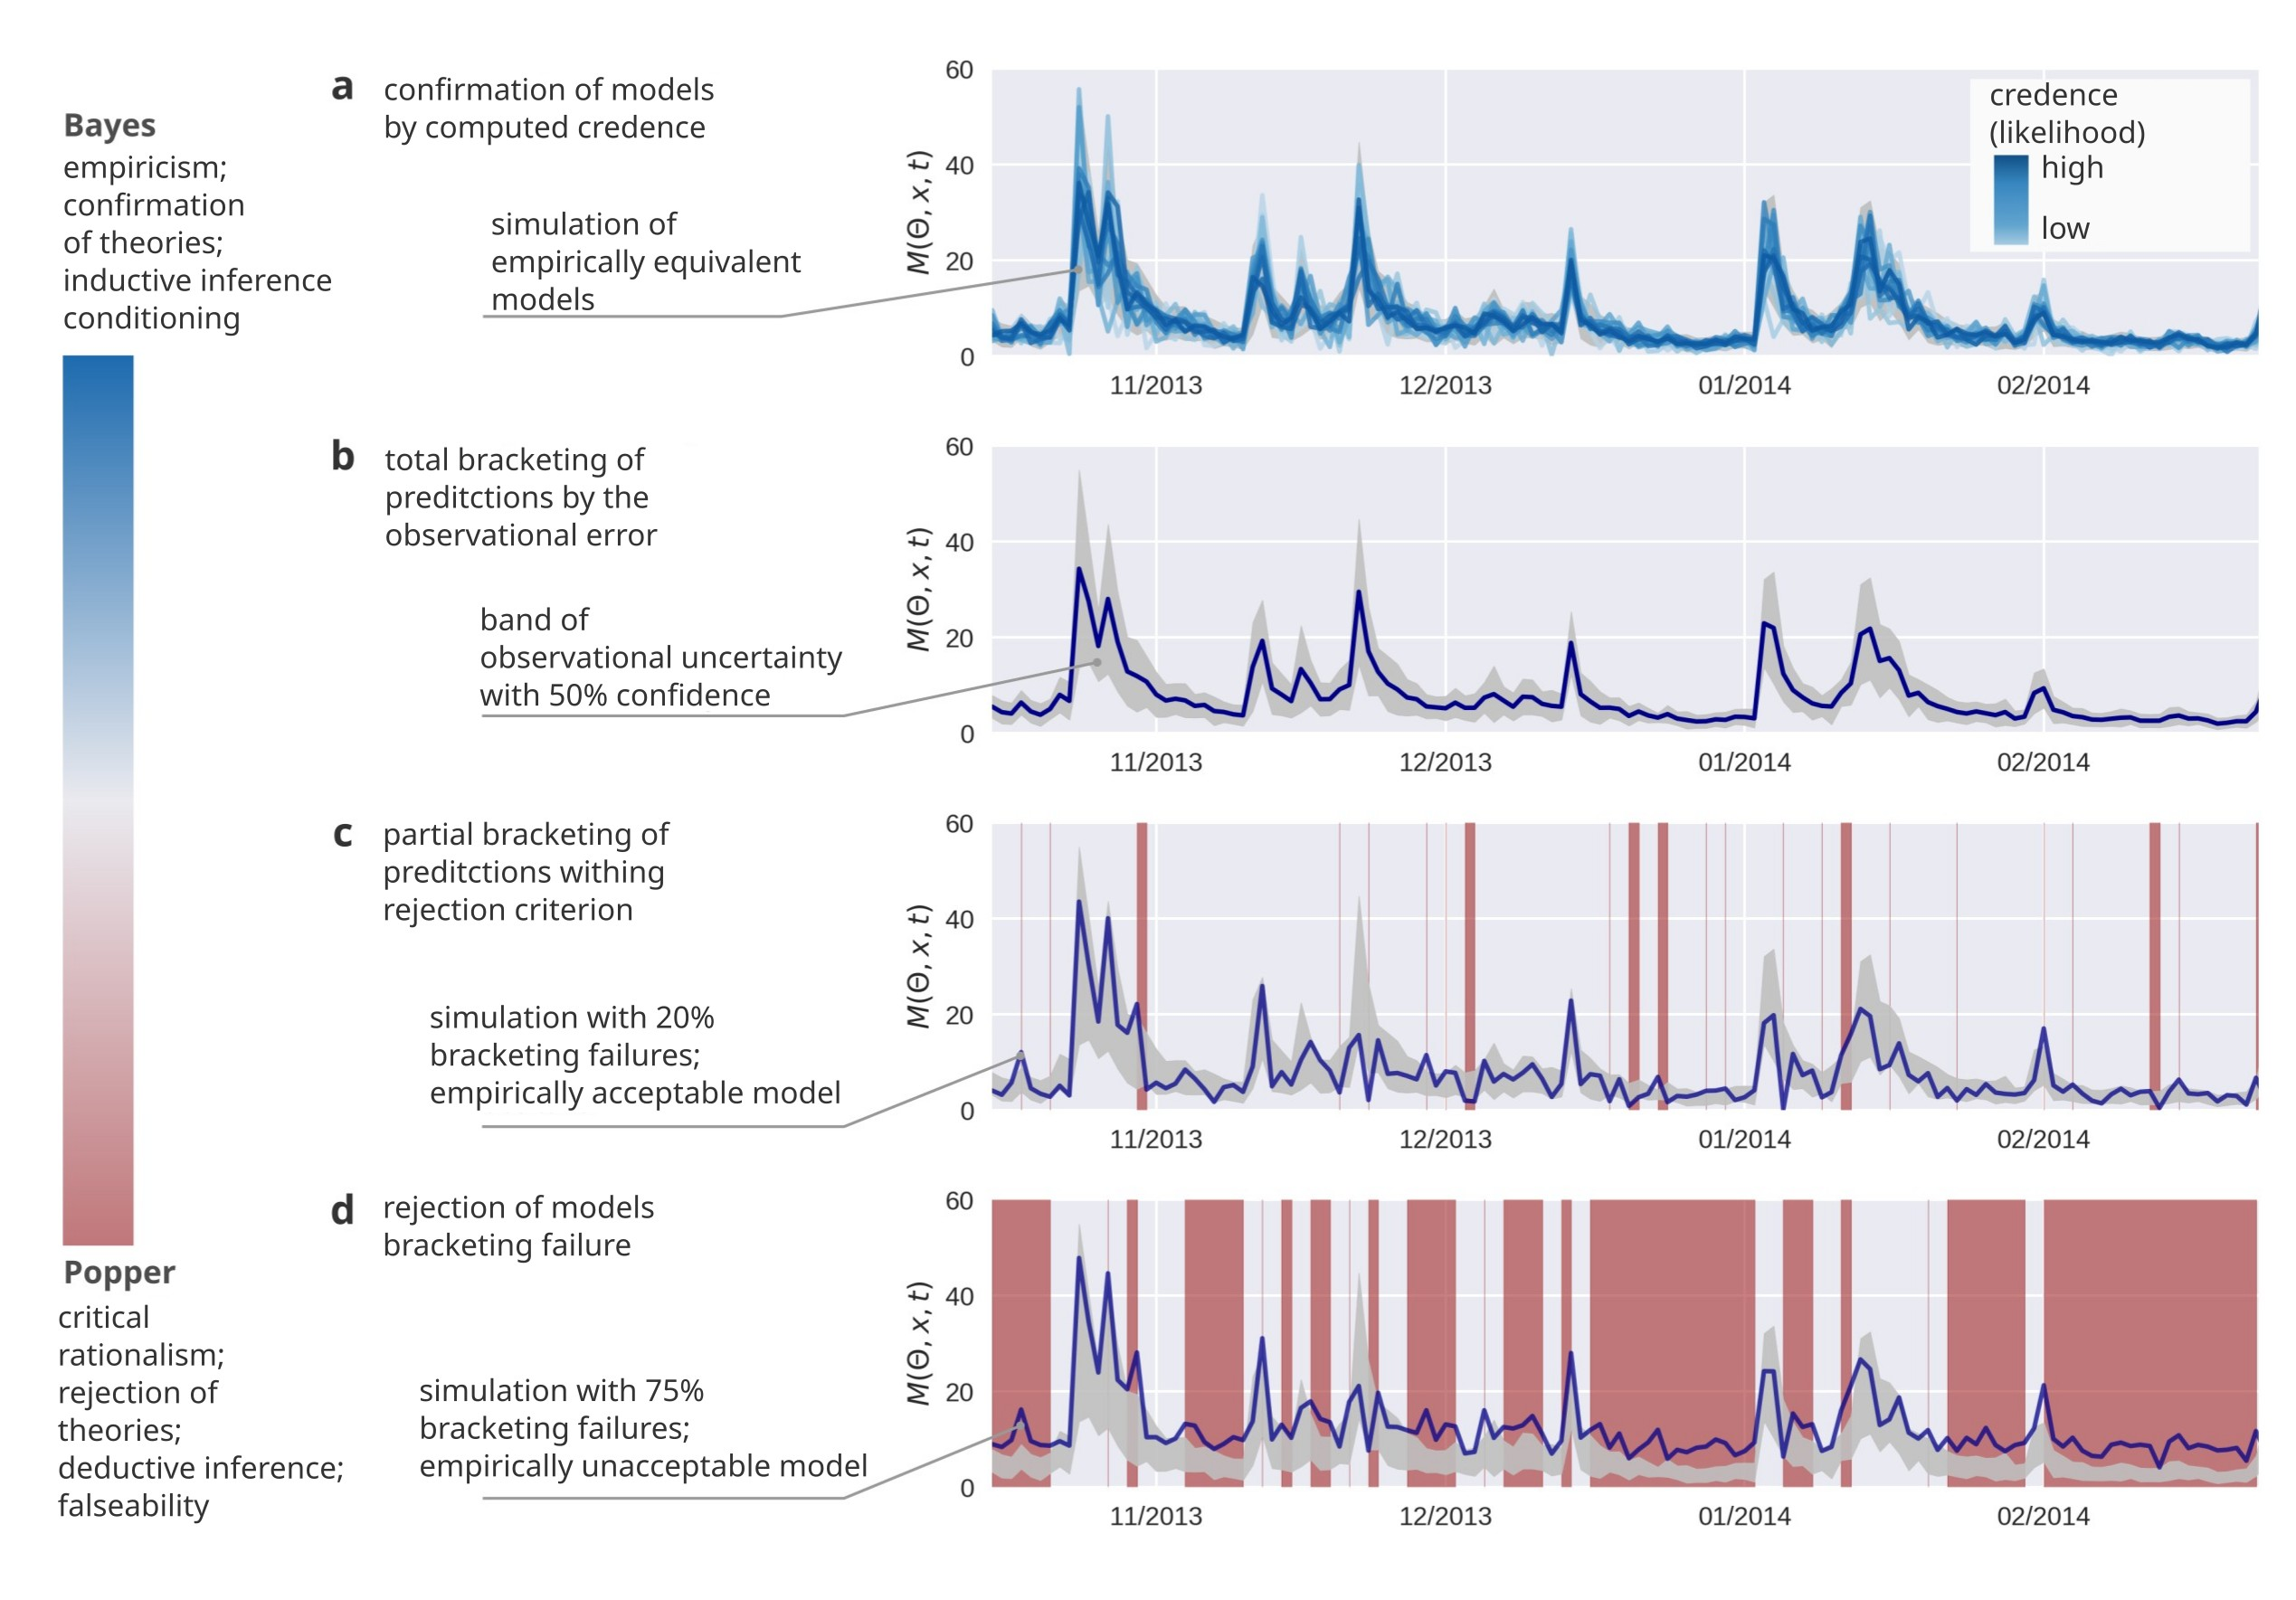
\includegraphics[width=0.95\linewidth]{fig_approach_en.jpg}		
	\caption[Instrumentalist approach to hydrological modeling]
	{\textbf{---\;Instrumentalist approach to hydrological modeling.}
        In this approach, both Bayes' confirmation and Popper's rejection are employed under the recognition of the \gls{problem-subdet} (equifinality). \;\textbf{a}\;---\;Confirmation of models through Bayesian \gls{conditioning}, where degrees of confirmation (informal \gls{likelihood} measures) are assigned to \gls{emp-eq-model}. In this case, all models are encapsulated by the observational uncertainty band within the pre-established rejection threshold.\;\textbf{b}\;---\;Total (no failures) encapsulation of a simulation (time series) by the \gls{error-obs} of the empirical evidence. In the illustrated case, the uncertainty band has a confidence level of 50\%. A more or less comprehensive band should be defined \textit{a priori}.\;\textbf{c}\;---\;Partial encapsulation (with 20\% failures) of a simulation by the \gls{error-obs}. As the band is at 50\% confidence, the failures are within the rejection threshold, and the \gls{model} can be considered empirically acceptable.\;\textbf{d}\;---\;Rejection of models due to insufficient encapsulation (75\% failures). In this case, the failures exceed the 50\% confidence level, and the \gls{model} must be considered empirically unacceptable.\;
	}
\label{fig:approach}  % use qualitative label			
\end{figure}

% encapsulation equation
\par With Equation \eqref{eq:total-error}, Keith Beven operationalizes an instrumentalist \gls{paradigma} for hydrological modeling that, beyond confirmation, \textit{allows for the rejection of models}. This approach follows the recommendations discussed by Albert Tarantola, to consider both the empiricist confirmation of Bayes and the rationalist rejection of Popper for a philosophically explicit approach to environmental modeling \cite{Tarantola2006}. In this line, the critique of the hegemonic modeling \gls{paradigma}, dominated by \gls{prag-realism}, is that model confirmation occurs at the cost of underestimating epistemic uncertainties, masking them as random error minimized through optimization techniques, as seen in Equation \eqref{eq:bayes-model}. This leads to the \textbf{\gls{problem-overfitting}} of models to the available data used. Through the conventional \textbf{\gls{proc-calib}}\footnote{Also referred to as the \textit{inverse problem}}, one reaches the (incorrect) conclusion that the adjusted \gls{model} identified is the only empirically adequate representation. On the other hand, the new instrumentalist approach, in Beven's words:

\begin{adjustwidth}{100pt}{0pt}
\medskip
\small (...) There is, however, another approach. That is to accept that it is very unlikely that our current model structures are truly realistic descriptions of the enviromental systems of interest so that there may indeed be many different models that can be shown to provide predictions that are acceptably consistent with whatever observed data are available. That is to treat the problem of identifiability as one of equifinality of model structures and parameter sets in reproducing the known behaviour of the system. -- Keith Beven (2009. p. 15) \cite{Beven2009}.
\medskip
\end{adjustwidth}

\begin{simplebox}[
    float=ht!,
    label={highlight_uncertainty_maps},
    nameref={Uncertainty Maps}
    ]{The impact of uncertainty on mapping priority actions}
    \footnotesize
    % first minipage
    \begin{minipage}[t]{\linewidth}  
    \par When applied under the instrumentalist paradigm, by admitting multiple empirically adequate solutions, hydrological models do not produce exact values of the simulated variables but rather intervals where confidence is higher or lower. For instance, from a population of suitable models, it is possible to simulate a \textbf{bundle of flow series}. Moving statistics on these time series can capture the central tendency, such as the mean, or the dispersion, such as the bands produced by lower and upper percentiles. However, when models simulate hydrological processes in a distributed manner in space, a \textbf{stack of maps} is generated, which can be somewhat difficult to visualize. One solution is to visualize centrality and dispersion on separate maps or synthesize an uncertainty index, such as a normalized coefficient of variation.
    \end{minipage}
    
    % second min
    \begin{minipage}[t]{\linewidth}
        \begin{minipage}[t]{\linewidth}
        \vspace*{5pt}
        	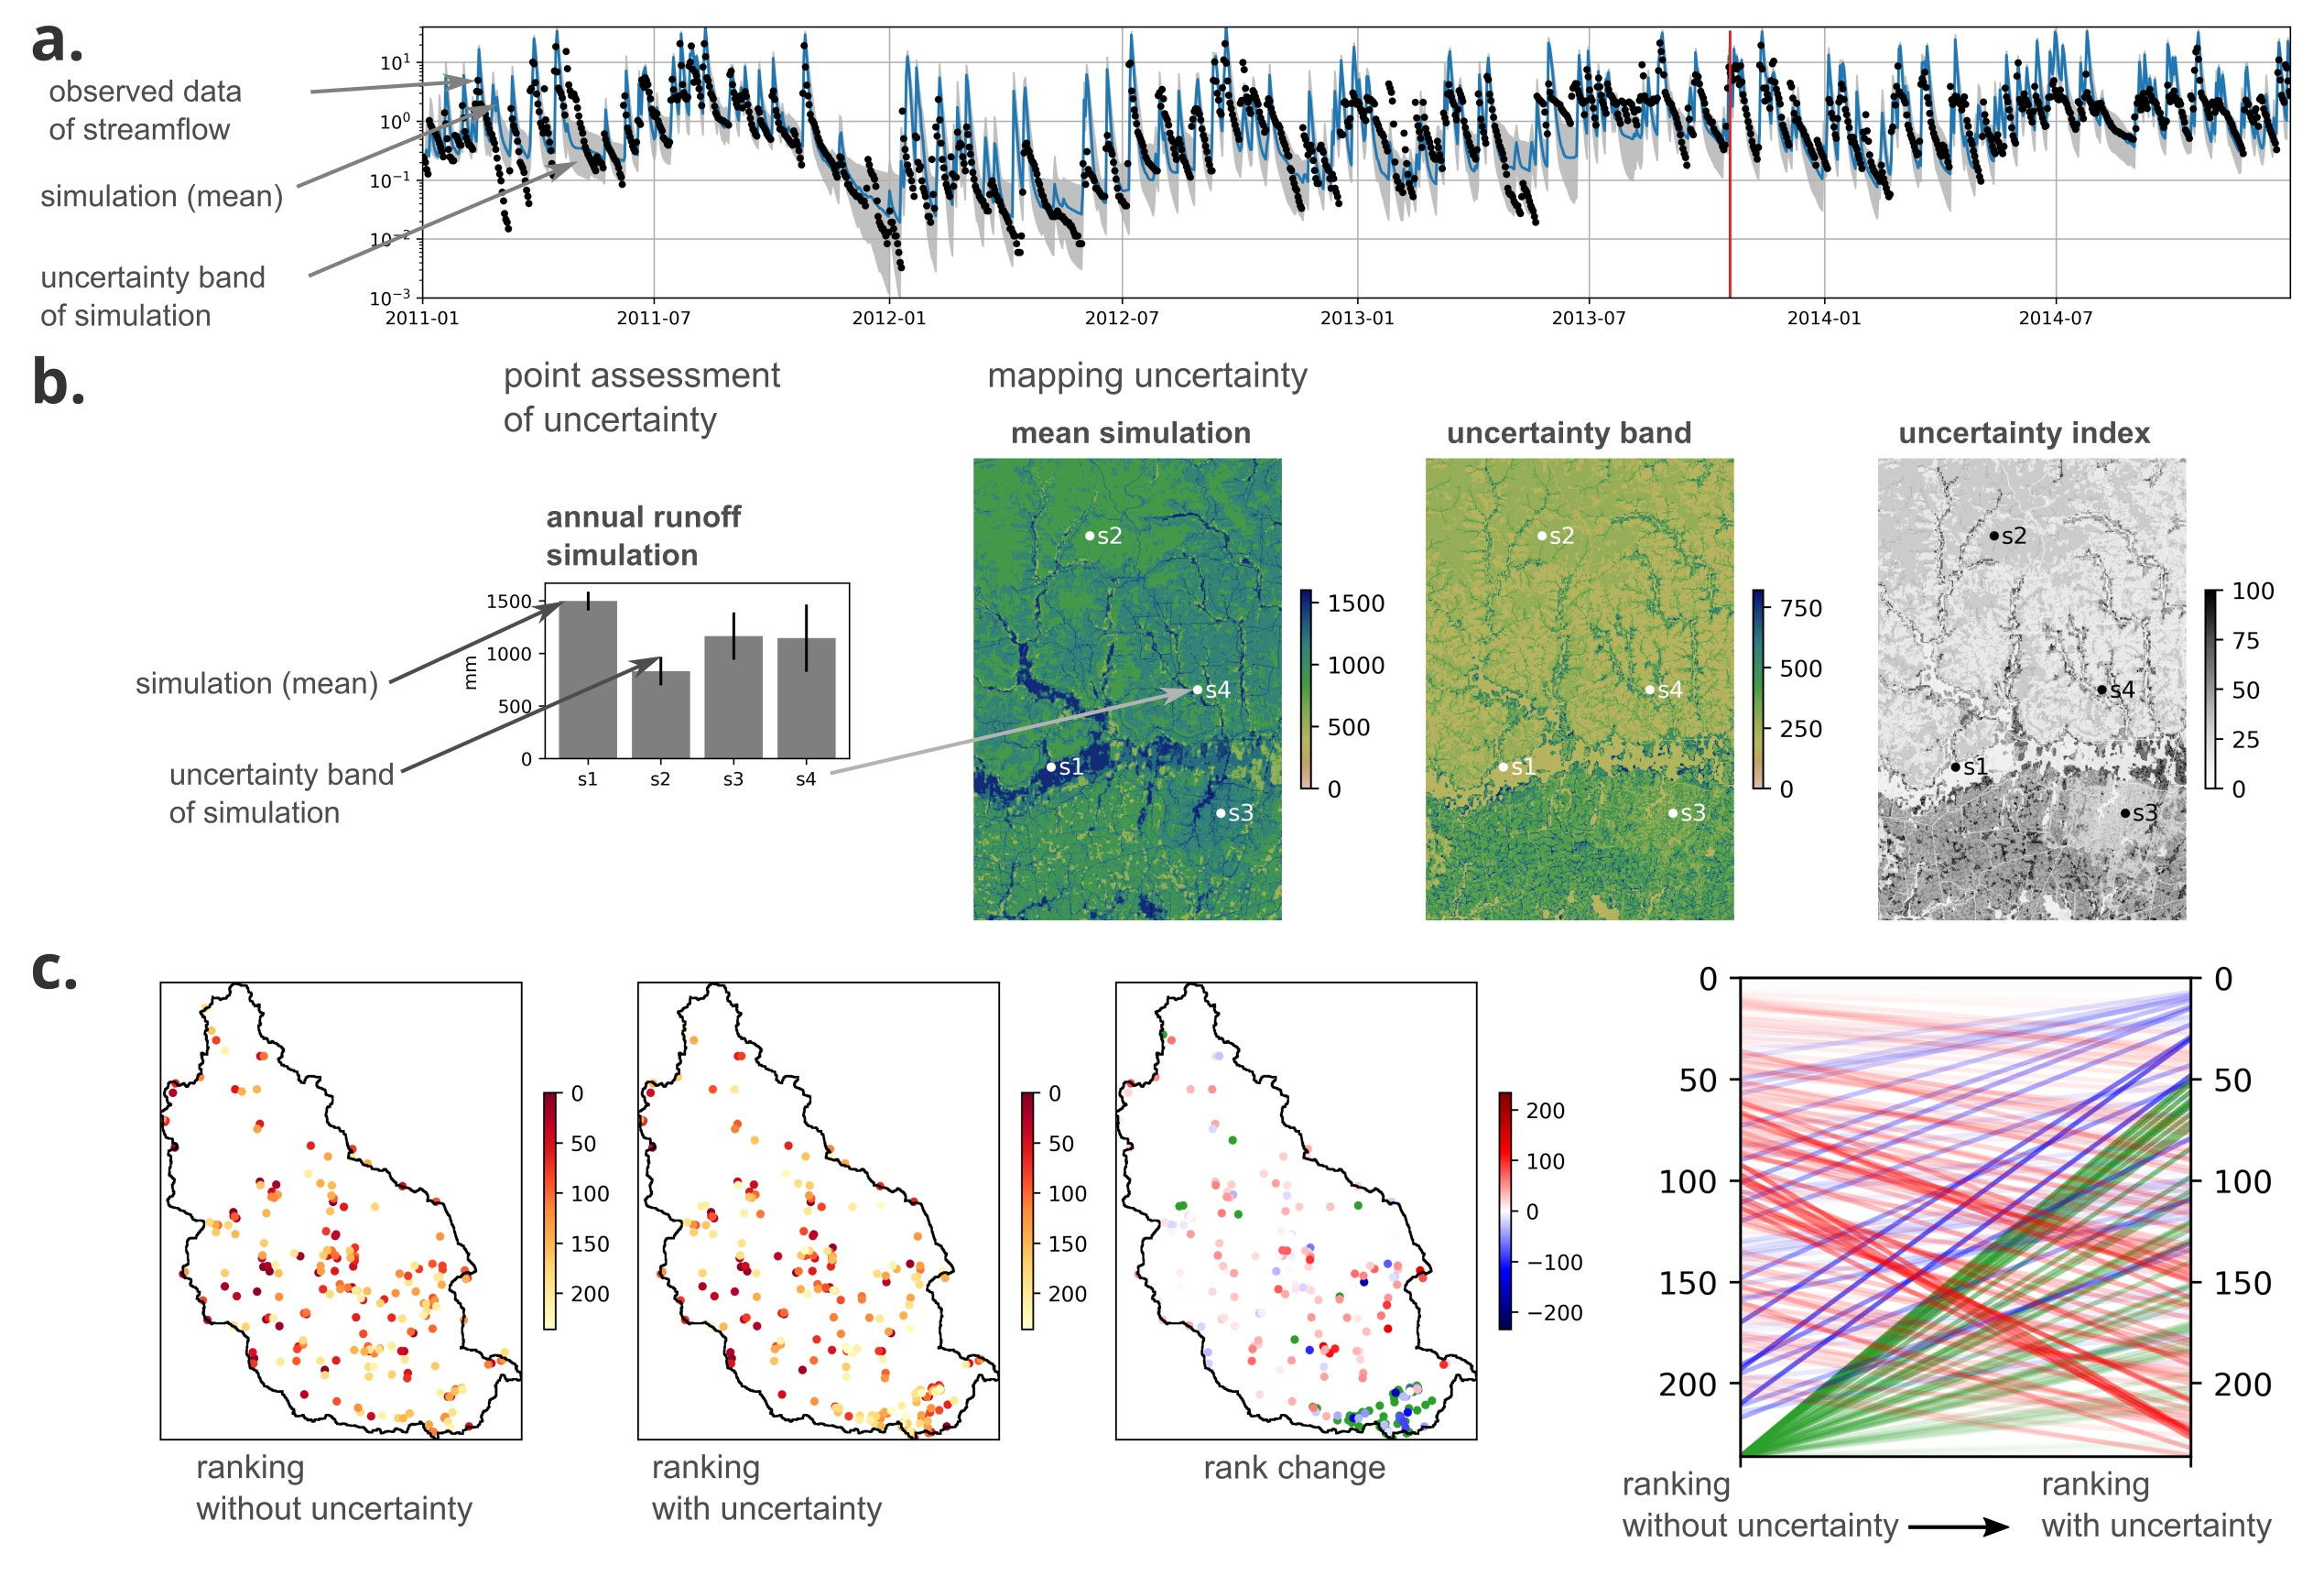
\includegraphics[width=\linewidth]{figs/fig_uncert_en.jpg}	
        	\captionof{figure}[Mapping priority areas considering uncertainties]{
                \textbf{---\;Mapping priority areas considering uncertainties in modeling}\;\textbf{a}\;---\;Expression of uncertainties over time through uncertainty bands.\;\textbf{b}\;---\;Expression of uncertainties in space by considering separate maps or a normalized uncertainty index\;\textbf{c}\;---\;Impact on the ranking of priority areas, comparison of ranking with and without uncertainties. 
        	}
            \label{fig:mapsuncer}  % use qualitative label	
        \vspace*{5pt}
        \end{minipage}
    \end{minipage}
    
    \begin{minipage}[t]{\linewidth}
    
    \par Since evidence-based policies need to account for empirical uncertainties, model uncertainty has been used as relevant information in identifying priority areas \cite{EVENSON2021}. This approach was articulated by me and my colleagues in Possantti et \textit{al.} (2023) \cite{Possantti2023a}, by employing a priority index weighted by uncertainty in regions $i$:
    \begin{equation}
        \label{eq:ip}
        \text{IP}_{i} = \frac{\sum_{i=1}^{N}\text{IU}_{i} * \text{IA}_{i} }{\sum_{i=1}^{N}\text{IU}_{i}} \quad \forall i
    \end{equation}
    Where $IP_{i}$ is the \textbf{priority index}; $IA$ is the \textbf{suitability index} chosen based on the central tendency, and; $IU$ is the \textbf{uncertainty index}. In other words, when prioritizing actions where there is greater surface runoff, the ranking of areas will be weighted by the modeling uncertainty. The results demonstrate that model uncertainty is not uniform in space, causing substantial impacts on ranking when considered by the prioritization formula.    
    
    \end{minipage}
\label{box:uncert}
\normalsize
\end{simplebox}


\noindent It is important to note that this new approach does not abandon the confirmation process through the Bayesian \gls{conditioning} of the posterior distribution of the \gls{parameters} $\Theta$. Although the \gls{eq-total-error} makes a formal treatment of the \gls{likelihood} $P(O|M)$ impossible, it remains possible to assign different degrees of conviction, or weights, to the \textbf{\gls{emp-eq-model}} through informal \gls{likelihood} measures $\mathcal{L}(O|M)$. The novelty of the approach lies in establishing that an \textbf{\gls{emp-acc-model}}\footnote{Keith Beven refers to empirically acceptable models as \textit{behavioral models}.} occurs when its structural error $\varepsilon_M$ is less than its \gls{error-obs} $\varepsilon_O + \varepsilon_{\Delta}$. Otherwise, the \gls{model} must be rejected. This implies that the predictions of any \gls{model} must be \textit{encapsulated} by a confidence interval defined \textit{a priori} as a rejection criterion. In other words, for a confidence level of $\alpha$\%, the \textbf{\gls{eq-bracketing}}:
\begin{linenomath*}
\begin{equation}
\label{eq:bracketing}
    O_{100-\alpha\%}(x, t) < M(\Theta, \Upsilon, \varepsilon_{\Upsilon}, x, t) < O_{\alpha\%}(x, t) \quad \forall \quad x, t
\end{equation}
\end{linenomath*}
must hold true with a frequency of at least $\alpha\%$; where $O_{100-\alpha\%}$ and $O_{\alpha\%}$ are the lower and upper thresholds of the confidence interval of the \gls{error-obs} at each sample point $x, t$. This approach has exactly the same structure as statistical \gls{hipotese} tests: 1) a rejection criterion is pre-defined by a confidence level $\alpha$\%; 2) a test statistic is calculated, in this case the encapsulation rate of the simulation, and; 3) the p-value of the test is evaluated, which in this case is the failure rate of encapsulation. If the p-value is greater than the confidence level, the \gls{model} should be rejected. On the other hand, all models that pass the minimum encapsulation test are considered empirically equivalent and can be confirmed based on \gls{likelihood} measures. Figure \ref{fig:approach} illustrates the approach for encapsulating a time series of any hydrological variable, but it is generally the discharge in a river section. It is noted that the pre-definition of the confidence level implies more or less comprehensive observational uncertainty bands. This fact introduces the following dilemma: when high certainty about predictions is desired, the observational band may be very wide, resulting in various empirically acceptable simulations and little precision in structural error. This creates the need to obtain more evidence, so that the observations themselves present narrow bands for high confidence levels. Another aspect that differs from the hegemonic \gls{paradigma}, which operates solely through confirmation, is that nothing prevents the eventual \textit{rejection of all tested models} by the \gls{eq-bracketing}. If this is the case, Beven emphasizes, a valuable opportunity arises to transform modeling into a learning process, forcing users to review both the \gls{aux-hyp} and the main \gls{hipotese}, that is, the very theoretical assumptions adopted in the conception of the modeled hydrological processes. Ultimately, total rejection imposes the need for new theories and explanations \cite{Beven2018}. Without this, the \gls{comunidade-cientifica} in this field will be forever trapped in the same paradigms. $\blacksquare$

\clearpage

\section{Chapter summary} \label{sec:epis:summary}

\par In this chapter, I aimed to establish the foundations of an instrumentalist philosophy for the application of hydrological models. The distinction between rationalism, with its emphasis on deduction, and empiricism, which values induction, was highlighted. From the empiricist side, I presented Bayesian epistemology, which proposes a gradual confirmation of hypotheses based on probabilities. From the rationalist perspective, I articulated the deductive rejection of theories, a stance defended by Karl Popper. In his thesis on scientific paradigms, Thomas Kuhn explains the alternation between periods of normal science and crises. The problem of underdetermination, raised by critics of scientific realism, is applied to hydrological modeling, culminating in an instrumentalist proposal that addresses epistemic uncertainty in the acceptance of empirically adequate models.

\begin{itemize}
    \item[$\blacksquare$] \textbf{The problem of justification}. There is a difficulty in justifying the truth of theories, in establishing definitive explanations for events and phenomena. On one hand, rationalists appeal to the use of \gls{infer-dedu}, which guarantees the truth of statements as long as their premises are true. On the other hand, empiricists prefer to use \gls{infer-indu}, which employs empirical evidence to generalize observed patterns.
    \item[$\blacksquare$] \textbf{Inductive confirmation of hypotheses}. Bayesian epistemology describes the process of empirical \gls{conditioning} to confirm hypotheses. By recognizing the existence of random noise in empirical observations, the truth of a \gls{hipotese} must be described as a \gls{grau-convic}, or probability. In this process, the probability distribution of hypotheses is incrementally adjusted through the application of Bayes' Theorem.
    \item[$\blacksquare$] \textbf{Deductive rejection of theories}. Karl Popper, when analyzing the Logic of scientific research, argues that the only safe way to acquire knowledge is through deductive refutation. In this sense, the role of empirical evidence is to test a \gls{hipotese} against counterexamples that prove its falsehood. For this reason, Popper claims that scientific theories must be falsifiable theories that allow for their own rejection.
    \item[$\blacksquare$] \textbf{Paradigms and the context of discovery}. Thomas Kuhn, by exploring the History of Science, eliminates the apparent contradiction between confirmation and rejection of theories. He argues that the dynamics of the \gls{comunidade-cientifica} plays a profound role in the production of knowledge, especially in the advent of paradigms. For him, confirmation occurs in periods of \gls{ciencia-normal}, while rejection predominates in crisis periods. Crisis periods end only when the competition of new ideas leads to a new \gls{paradigma}.
    \item[$\blacksquare$] \textbf{The problem of underdetermination}. \gls{realism-sci} is deeply questioned by Bas van Fraassen and Nancy Cartwright. They establish an instrumentalist perspective, where the goal of Science is solely to produce empirically adequate theories. This mainly stems from the instance of unobservable entities, which renders theories underdetermined by the evidence. A version of this occurs in hydrological modeling due to many modeled processes being practically unobservable -- the so-called \gls{problem-equifinal}. In this line, Keith Beven proposes an instrumentalist \gls{paradigma} for the application of models, allowing for the rejection of models based on the encapsulation test of predictions by observational uncertainty. Models that pass the test are deemed empirically acceptable and equivalent.
\end{itemize}


\end{document}